\documentclass[11pt]{article}
\usepackage[T1]{fontenc}
\usepackage[utf8]{inputenc}
\usepackage{fourier}
\usepackage[scaled=0.875]{helvet}
\renewcommand{\ttdefault}{lmtt}
\usepackage{amsmath,amssymb}
\usepackage{makeidx}
\makeindex
\usepackage{fancybox}
\usepackage[normalem]{ulem}
\usepackage{pifont}
\newcommand{\textding}[1]{\text{\ding{#1}}}
\usepackage{lscape}
\usepackage{tabularx,booktabs}
\usepackage{scratch}
\usepackage{textcomp}
\usepackage{enumitem}
\usepackage{multicol}
\usepackage{multirow}
\newcommand{\euro}{\eurologo{}}
%Tapuscrit : Denis Vergès 
\usepackage{pst-eucl}
\usepackage{diagbox}% à mettre après pst-eucl
\usepackage{graphicx,pstricks,pst-plot,pst-grad,pst-node,pst-text,pstricks-add}
\usepackage{pstricks-add}
\usepackage{pgf,tikz,pgfplots}
\usetikzlibrary{patterns,calc,decorations.pathmorphing}
\newcommand{\R}{\mathbb{R}}
\newcommand{\N}{\mathbb{N}}
\newcommand{\D}{\mathbb{D}}
\newcommand{\Z}{\mathbb{Z}}
\newcommand{\Q}{\mathbb{Q}}
\newcommand{\C}{\mathbb{C}}
\usepackage[left=3.5cm, right=3.5cm, top=2.2cm, bottom=2cm]{geometry}
\setlength\headheight{13.7pt}
\newcommand{\vect}[1]{\overrightarrow{\,\mathstrut#1\,}}
\renewcommand{\theenumi}{\textbf{\arabic{enumi}}}
\renewcommand{\labelenumi}{\textbf{\theenumi.}}
\renewcommand{\theenumii}{\textbf{\alph{enumii}}}
\renewcommand{\labelenumii}{\textbf{\theenumii.}}
\def\Oij{$\left(\text{O}~;~\vect{\imath},~\vect{\jmath}\right)$}
\def\Oijk{$\left(\text{O}~;~\vect{\imath},~\vect{\jmath},~\vect{k}\right)$}
\def\Ouv{$\left(\text{O}~;~\vect{u},~\vect{v}\right)$}
\usepackage{fancyhdr}
\usepackage[dvips,colorlinks=true,pdfstartview=FitV,linkcolor=blue,citecolor=blue,urlcolor=blue]{hyperref}
\hypersetup{%
pdfauthor = {APMEP},
pdfsubject = {Brevet},
pdftitle = {Année 2021},
allbordercolors = white,
pdfstartview=FitH}
\usepackage[french]{babel}
\usepackage[np]{numprint}
\usepackage{colortbl}
%\usetikzlibrary{backgrounds}
%\usetikzlibrary{calc,shapes.arrows,decorations.pathreplacing}
\begin{document}
\setlength\parindent{0mm}
\rhead{\textbf{A. P{}. M. E. P{}.}}
\lhead{\small L'intégrale 2021}

\pagestyle{fancy}
\thispagestyle{empty}
\begin{center} {\huge \textbf{\decofourleft~Brevet des collèges  2021~\decofourright\\\vspace{1cm} L'intégrale de juin 2021 à novembre 2021}}

\vspace{1cm}

Pour un accès direct cliquez sur les liens {\Large \textcolor{blue}{bleus}}
\end{center}
 
\begin{tabularx}{\linewidth}{>{\Large}X}

\hyperlink{AmeriqueduNord}{Amérique du Nord 4 juin 2021}\dotfill \pageref{AmeriqueduNord} \\
\hyperlink{Etranger}{Centres étrangers  14 juin 2021} \dotfill \pageref{Etranger} \\
\hyperlink{Asie}{Asie 21 juin  2021} \dotfill \pageref{Asie}  \\
\hyperlink{Asie_secours}{Asie (secours) 21 juin  2021} \dotfill \pageref{Asie_secours}  \\
\hyperlink{Polynesie}{Polynésie 25 juin 2021} \dotfill \pageref{Polynesie} \\
\hyperlink{Metropole}{Métropole, La Réunion, Antilles--Guyane 28 juin 2021} \dotfill \pageref{Metropole}\\
\hyperlink{Metropolesep}{Métropole, La Réunion, Antilles--Guyane 20 sept. 2021} \dotfill \pageref{Metropolesep} \\
\hyperlink{AmeriqueSud}{Amérique du Sud 23 novembre 2021}  \dotfill \pageref{AmeriqueSud} \\
\hyperlink{Caledoniedec}{Nouvelle-Calédonie 7 décembre 2021}  \dotfill \pageref{Caledoniedec}
\end{tabularx}

\vspace{1cm}

\hyperlink{Index}{À la fin index des notions abordées}
\newpage
 ~
\newpage
%%%%%%%%%%%%%   Amérique du Nord 3 juin 2021
\hypertarget{AmeriqueduNord}{}

\label{AmeriqueduNord}

\rhead{\textbf{A. P{}. M. E. P{}.}}
\lhead{\small Brevet des collèges}
\lfoot{\small{Amérique du Nord}}
\rfoot{\small 3 juin 2021}

\marginpar{\rotatebox{90}{\textbf{A. P{}. M. E. P{}.}}}
\pagestyle{fancy}
\thispagestyle{empty}

\begin{center}\textbf{Durée : 2 heures}

\vspace{0,5cm}

{\Large\textbf{\decofourleft~Diplôme national du Brevet
Amérique du Nord~\decofourright}}\\[6pt]
{\Large \textbf{3 juin 2021}}


\medskip

\emph{L'usage de calculatrice avec mode examen activé est autorisé.\\
L'usage de calculatrice sans mémoire \og type collège \fg{} est autorisé}

\end{center}

\vspace{0,5cm}

\textbf{{\large \textsc{Exercice 1}} \hfill 26 points}

Pour chacune des six affirmations suivantes, indiquer sur la copie, si elle est vraie ou fausse.

\medskip

\textbf{On rappelle que chaque réponse doit être justifiée.}

\begin{enumerate}[itemsep=5mm]
	\item On considère la fonction $f$ définie par $f(x) = 3x - 7$\index{fonction affine}
	
	\textbf{Affirmation \no 1 :} \og{}L’image par $f$ du nombre $- 1$ est 2 \fg{}.
	
	\item On considère l'expression $\mathrm{E} = (x - 5)(x + 1)$.
	
	\textbf{Affirmation \no 2 :} \og{} L'expression $ \mathrm{E} $ a pour forme développée et réduite $x^2 - 4x - 5 $\fg{}.\index{développement}
	
	\item $n$ est un nombre entier positif.
	
	\textbf{Affirmation \no 3 :} \og{}lorsque $n$ est égal à 5, le nombre $2^n +1$ est un nombre premier \fg{}.\index{nombre premier}
	
	\item On a lancé 15 fois un dé à six faces numérotées de 1 à 6 et on a noté les fréquences d'apparition dans le tableau ci-dessous :\index{fréquence}
	
	\smallskip
	\begin{tabularx}{\linewidth}{|m{3.5cm}|*{6}{>{\centering \arraybackslash}X|}} \hline
Numéro de la face apparente & 1& 2& 3& 4& 5& 6 \\ \hline
Fréquence d'apparition&$\dfrac{3}{15}$&$\dfrac{4}{15}$&$\dfrac{5}{15}$&$\dfrac{2}{15}$&$\dfrac{1}{15}$ &\dots\rule[-3mm]{0mm}{9mm}\\ \hline
	\end{tabularx}
	
	\smallskip
	
	\textbf{Affirmation \no 4 :} \og{}la fréquence d'apparition du 6 est 0 \fg{}.
	
	\item On considère un triangle RAS rectangle en S.
	
Le côté [AS] mesure $80$~cm et l'angle $\widehat{\mathrm{ARS}} $ mesure $26\degres$.
	
	\textbf{Affirmation \no 5 :} le segment [RS] mesure environ $164$~cm.
	
	\item Un rectangle ABCD a pour longueur 160 cm et pour largeur $95$~cm.
	
	\textbf{Affirmation \no 6 :} les diagonales de ce rectangle mesurent exactement $186$~cm.
\end{enumerate}

\bigskip

\textbf{{\large \textsc{Exercice 2}} \hfill 21 points}

Une athlète a réalisé un triathlon d’une longueur totale de 12,9 kilomètres. Les trois épreuves se déroulent dans l’ordre suivant :
	
	\begin{center}
		\begin{tabularx}{14 cm}{|*{3}{>{\centering \arraybackslash}X|}} \hline
		Épreuve \tikz[baseline=(x.base)]{\draw (0,0) circle (8pt) node (x) {1};}\rule{0pt}{14pt} :     & Épreuve \tikz[baseline=(x.base)]{\draw (0,0) circle (8pt) node (x) {2};} :     & Épreuve \tikz[baseline=(x.base)]{\draw (0,0) circle (8pt) node (x) {3};} : \\
		Natation          & Cyclisme          & Course à pied. \\
		Distance = 400 m  &                   & Distance = 2,5 km\\ \hline
		\end{tabularx}
	\end{center}

Entre deux épreuves, l’athlète doit effectuer sur place un changement d'équipement.
	
	Le graphique ci-dessous représente la distance parcourue (exprimée en kilomètre) par l’athlète, en fonction du temps de parcours (exprimé en minute) de l’athlète pendant son triathlon.
	
	\begin{center}
		\begin{tikzpicture}[x=1.8mm,y=9mm,> = latex]
			\draw [gray,xstep=5,ystep=1] (0,0) grid (65,15);
			\draw[<->] (0,15.2) node [above right] {\textbf{Distance en kilomètre}}--(0,0)--(66,0) node[shift={(0,-1)}, left] {\textbf{Temps en minute}};
			\foreach \x in {5,10,...,60}{
				\draw (\x,2pt)--(\x,-2pt) node [below] {\x};}
				%%%%%%%%
\foreach \y in {1,2,...,15}{
\draw (2pt,\y)--(-2pt,\y) node [left] {\y};}
\node at (0,0) [below left] {0};
	
				%%%%%%%%
			\draw[line width=0.8pt] (0,0)--(14,0.4)--(15,0.4)--(42,10.4)--(44,10.4)--(56,12.9);
			\foreach \c in {(14,0.4),(15,0.4),(42,10.4),(44,10.4),(56,12.9)}
				\draw[shift=\c,line width=0.8pt] (-3pt,0)--(3pt,0) (0,3pt)--(0,-3pt);
			\draw[fill = white] (7,.8) circle (8pt) node (x) {1};
			\draw[fill = white] (27.2,6.1) circle (8pt) node (y) {2};
			\draw[fill = white] (52.5,11.3) circle (8pt) node (z) {3};
			\draw (42,10.4) node[above left] {M};
			\draw[<-](14,0.6)--(14,5) node[text width=38 mm, align = center, fill=white, draw] {Premier changement d'équipement};
			\draw[<-](43,10.6)--(43,14.2) node[text width=38 mm, align = center, fill=white, draw] {Deuxième changement d'équipement};
		\end{tikzpicture}
	\end{center}	

Le point M a pour abscisse 42 et pour ordonnée 10,4.
	
À l’aide du tableau ci-dessus ou par lecture du graphique ci-dessus avec la précision qu’il permet, répondre aux questions suivantes, en justifiant la démarche.\index{lecture graphique}

\medskip
	
	\begin{enumerate}
		\item Au bout de combien de temps l’athlète s’est-elle arrêtée pour effectuer son premier changement d'équipement ?
		\item Quelle est la longueur, exprimée en kilomètre, du parcours de l'épreuve de cyclisme ?
		\item En combien de temps l’athlète a-t-elle effectué l'épreuve de course à pied ?
		\item Parmi les trois épreuves, pendant laquelle l’athlète a été la moins rapide ?
		\item On considère que les changements d'équipement entre les épreuves font partie du triathlon.
		
La vitesse moyenne de l’athlète sur l’ensemble du triathlon est-elle supérieure à 14 km/h ?
	\end{enumerate}
	
\newpage
	
\textbf{{\large \textsc{Exercice 3}} \hfill 16 points}
	
\begin{minipage}[t]{7 cm}
		\emph{Dans cet exercice, aucune justification n'est demandée.}

On a construit un carré ABCD. 

\smallskip

On a construit le point O sur la droite (DB), à l'extérieur du segment [DB] et tel que : 

OB = AB.

\smallskip

Le point H est le symétrique de D par rapport à O.
		
\bigskip
		
On a obtenu la figure ci-contre en utilisant plusieurs fois la même rotation de centre O et d'angle $45\degres$.\index{rotation}
		
		\bigskip
		
		La figure obtenue est symétrique par rapport à l’axe
		(DB) et par rapport au point O.\index{symétrie centrale}
\end{minipage}
	\hfill
	\begin{tikzpicture}[baseline={(D)}]
		\foreach \a in {0,45,...,315}
			\draw [line width=0.8pt] (0+\a:1.414)--++(-45+\a:1.414)--++(45+\a:1.414)--++(135+\a:1.414)--cycle;
		\foreach \a/\l in {2/E,3/F,4/G,6/I,7/J,8/K}
			\draw (135-\a*45:2.414) circle (7pt) node {\a}
			(135-\a*45:3.7) node{\l};
		\draw (0.4,2.414) circle (7pt) node {1};
		\draw (-0.4,-2.414) circle (7pt) node {5};
		\draw[line width=0.8pt] (0,-4)--(0,4) 
		(-3pt,-3pt)--(3pt,3pt) (-3pt,3pt)--(3pt,-3pt) (1pt,0)node[right] {O};
		\node (A) at (67.5:2.6) [above right]{A};
		\node (B) at (90:1.414) [below right] {B};
		\node (C) at (112.5:2.6) [above left] {C};
		\node (D) at (90:3.7) [right] {D};
		\node (H) at (-90:3.7) [left] {H};
	\end{tikzpicture}

	\begin{enumerate}
		\item Donner deux carrés différents, images l’un de l’autre par la symétrie axiale d’axe (DB).\index{symétrie axiale}
		
		\item Le carré \tikz[baseline=(x.base)]{\draw (0,0) circle (7pt) node (x) {3};} est-il l’image du carré \tikz[baseline=(x.base)]{\draw (0,0) circle (7pt) node (x) {8};} par la symétrie centrale de centre O ?
		
		\item On considère la rotation de centre O qui transforme le carré \tikz[baseline=(x.base)]{\draw (0,0) circle (7pt) node (x) {1};} en le carré \tikz[baseline=(x.base)]{\draw (0,0) circle (7pt) node (x) {2};}.
		
		Quelle est l’image du carré \tikz[baseline=(x.base)]{\draw (0,0) circle (7pt) node (x) {8};} par cette rotation ?
		
		\item On considère la rotation de centre O qui transforme le carré \tikz[baseline=(x.base)]{\draw (0,0) circle (7pt) node (x) {2};} en le carré \tikz[baseline=(x.base)]{\draw (0,0) circle (7pt) node (x) {5};}.
		
		Préciser l’image du segment [EF] par cette rotation.
	\end{enumerate}

\bigskip

\textbf{{\large \textsc{Exercice 4}} \hfill  16 points}

	\begin{minipage}{12cm}
		\emph{Dans cet exercice, aucune justification n'est demandée.}
		
		On dispose d’un tableau carré ci-contre partagé en neuf cases blanches de mêmes dimensions qui constituent un motif.
	\end{minipage}
	\hfill
	\begin{tikzpicture}[x=6mm,y=6mm, baseline={(current bounding box.center)}]
		\foreach \xy/\c in {(0,0)/white,(1,0)/white,(2,0)/white,
							(0,1)/white,(1,1)/white,(2,1)/white,
							(0,2)/white,(1,2)/white,(2,2)/white}
			\draw[fill=\c, shift={\xy}] (0,0) rectangle (1,1);
	\end{tikzpicture}
		
	\medskip
	
Quatre instructions A, B, C et E permettent de changer l'aspect de certaines cases, lorsqu'on applique ces instructions. Ainsi :
	
	\begin{tabularx}{\linewidth}{| >{\centering \arraybackslash}m{2cm} | m{8cm} | >{\centering \arraybackslash}X |} \hline
		Instruction & Descriptif & Effet de l'instruction   \\ \hline
		A &   La case centrale du motif est noircie.  & 
		\begin{tikzpicture}[x=6mm,y=6mm, baseline={(current bounding box.center)}]
			\clip (-0.2,-0.2) rectangle (3.2,3.2);
			\foreach \xy/\c in {(0,0)/white,(1,0)/white,(2,0)/white,
				(0,1)/white,(1,1)/gray!50,(2,1)/white,
				(0,2)/white,(1,2)/white,(2,2)/white}
			\draw[fill=\c, shift={\xy}] (0,0) rectangle (1,1);
		\end{tikzpicture}  \\ \hline
		B &   Dans le motif, la case en bas à gauche et la case en haut à droite sont noircies. & 
				\begin{tikzpicture}[x=6mm,y=6mm, baseline={(current bounding box.center)}]
			\clip (-0.2,-0.2) rectangle (3.2,3.2);
			\foreach \xy/\c in {(0,0)/gray!50,(1,0)/white,(2,0)/white,
				(0,1)/white,(1,1)/white,(2,1)/white,
				(0,2)/white,(1,2)/white,(2,2)/gray!50}
			\draw[fill=\c, shift={\xy}] (0,0) rectangle (1,1);
		\end{tikzpicture}  \\ \hline
		
		C &   Dans le motif, la case médiane à gauche et la case médiane à droite sont noircies. & 
				\begin{tikzpicture}[x=6mm,y=6mm, baseline={(current bounding box.center)}]
			\clip (-0.2,-0.2) rectangle (3.2,3.2);
			\foreach \xy/\c in {(0,0)/white,(1,0)/white,(2,0)/white,
				(0,1)/gray!50,(1,1)/white,(2,1)/gray!50,
				(0,2)/white,(1,2)/white,(2,2)/white}
			\draw[fill=\c, shift={\xy}] (0,0) rectangle (1,1);
		\end{tikzpicture}  \\ \hline
		
		
		E &  Les couleurs du motif sont inversées: les cases blanches deviennent noires et les les cases noires deviennent blanches.&
				\begin{tikzpicture}[x=6mm,y=6mm, baseline={(current bounding box.center)}]
			\clip (-0.2,-0.2) rectangle (3.2,3.2);
			\draw[] (0,0) rectangle (3,3) ;
			\node (t) at (1.5,1.5) [text width=1.5cm, align=center] {Inverser\\ les\\ couleurs};
		\end{tikzpicture}  \\ \hline

	\end{tabularx}

\smallskip

\emph{Remarque} : si une case du motif est déjà noire et une instruction demande de la noircir, alors cette case ne change pas de couleur et reste noire à la suite de cette instruction.
	
\smallskip
	
\emph{Exemples} : à partir d’un motif dont toutes les cases sont blanches:
	
		\begin{tabularx}{\linewidth}{X c @{\hspace{5mm}}|@{\hspace{5mm}} X c} 
		la suite d'instructions A C permet d'obtenir ce motif &
		\begin{tikzpicture}[x=6mm,y=6mm, baseline={(current bounding box.center)}]
			\foreach \xy/\c in {(0,0)/white,(1,0)/white,(2,0)/white,
								(0,1)/gray!50,(1,1)/gray!50,(2,1)/gray!50,
								(0,2)/white,(1,2)/white,(2,2)/white}
				\draw[fill=\c, shift={\xy}] (0,0) rectangle (1,1);

		\end{tikzpicture}&
		la suite d'instructions A C E permet d'obtenir ce motif &
		\begin{tikzpicture}[x=6mm,y=6mm, baseline={(current bounding box.center)}]
			\foreach \xy/\c in {(0,0)/gray!50,(1,0)/gray!50,(2,0)/gray!50,
								(0,1)/white,(1,1)/white,(2,1)/white,
								(0,2)/gray!50,(1,2)/gray!50,(2,2)/gray!50}
					\draw[fill=\c, shift={\xy}] (0,0) rectangle (1,1);
		\end{tikzpicture}\\		
	\end{tabularx}

\medskip

Pour chacune des questions suivantes, on dispose au départ d’un motif dont toutes les cases sont blanches.
	
	\begin{enumerate}
		\item Représenter le motif obtenu avec la suite d'instructions A B.
		
		\item \begin{minipage}[t]{11 cm}
Parmi les quatre propositions suivantes, deux propositions permettent d'obtenir le motif ci-contre. Lesquelles ?
			
			\smallskip 
			
\begin{tabularx}{\linewidth}{*{2}{>{\bfseries Proposition \no }l <{ :} @{~} X}}
1 & A B C   & 3 & B C E C\\ [6pt]
2 & C E     & 4 & C A E A\\
\end{tabularx}
		\end{minipage}
		\hfill
		\begin{tikzpicture}[x=6mm,y=6mm, baseline={(0,1.6)}]
			\foreach \xy/\c in {(0,0)/gray!50,(1,0)/gray!50,(2,0)/gray!50,
								(0,1)/white,(1,1)/gray!50,(2,1)/white,
								(0,2)/gray!50,(1,2)/gray!50,(2,2)/gray!50}
				\draw[fill=\c, shift={\xy}] (0,0) rectangle (1,1);
		\end{tikzpicture}
		
		\item \begin{minipage}[t]{11 cm}
Donner une suite d'instructions qui permet d'obtenir le motif ci-contre.	
		\end{minipage}
		\hfill
%		\begin{tikzpicture}[x=6mm,y=6mm, baseline={(0,0.8)}]
%			\foreach \xy/\c in {(0,0)/gray!50,(1,0)/gray!50,(2,0)/white,
%								(0,1)/gray!50,(1,1)/white,(2,1)/gray!50,
%								(0,2)/white,(1,2)/gray!50,(2,2)/gray!50}
%			\draw[fill=\c, shift={\xy}] (0,0) rectangle (1,1);
%		\end{tikzpicture}
\begin{tikzpicture}[x=6mm,y=6mm, baseline={(0,0.8)}]
			\foreach \xy/\c in {(0,0)/white,(1,0)/gray!50,(2,0)/gray!50,
								(0,1)/gray!50,(1,1)/white,(2,1)/gray!50,
								(0,2)/gray!50,(1,2)/gray!50,(2,2)/white}
			\draw[fill=\c, shift={\xy}] (0,0) rectangle (1,1);
		\end{tikzpicture}
	\end{enumerate}

\bigskip

\textbf{{\large \textsc{Exercice 5}} \hfill  21 points}

\medskip

On souhaite rénover une salle de bain qui a la forme d’un parallélépipède rectangle. Il faut coller du papier peint sur les quatre murs. On n’en colle pas sur la porte, ni sur la fenêtre.
	
Voici un schéma de la salle de bain, les dimensions sont exprimées en mètre :
	
\begin{center}
	\begin{tikzpicture}[x=0.9cm,y=0.9cm,> = latex]
		\draw  (0,0) rectangle (9.6,6.1)
			   (2.3,0) rectangle (4.9,4.9)	
			   (0,6.1)--(4,9)--(13.7,9)--(13.7,2.9)--(9.6,0)
			   (9.6,6.1)--(13.7,9);
		\draw[dash pattern=on 2mm off 1.5mm] 
				(0,0)--(4,2.9)--(13.7,2.9)
				(4,2.9)--(4,9)
				(6.4,5.5) rectangle (9.3,8)
				(7.85,5.5)--(7.85,8)
				(6.4,6.75)--(9.3,6.75);
		\draw[<->, shift={(0,-0.25)}] (0,0)--(9.6,0)
		node[below,pos=0.5]{3,50};
		\draw[<->, shift={(-57:0.25)}] (9.6,0)--(13.7,2.9)
		node[below right,pos=0.5]{2,50};
		\draw[<->, shift={(0.25,0)}] (13.7,2.9)--(13.7,9)
		node[right,pos=0.5]{2,50};
		\draw[<->, shift={(-0.25,0)}] (2.3,0)--(2.3,4.9)
		node[left,pos=0.5]{2,10};
		\draw[<->, shift={(0,0.25)}] (2.3,4.9)--(4.9,4.9)
		node[above,pos=0.5]{0,80};
		\draw[<->, shift={(-0.25,0)}] (6.4,5.5)--(6.4,8)
		node[left,pos=0.5]{1,20};
		\draw[<->, shift={(0,0.25)}] (6.4,8)--(9.3,8)
		node[above,pos=0.5]{1,60};
	\end{tikzpicture}
\end{center}
	
	On dispose des informations suivantes :
	
	\fbox{\rule[-2.1cm]{0mm}{4.4cm}\begin{minipage}{0.53\linewidth}
			Prix du papier peint :
			
			\begin{itemize}[label=\textbullet,leftmargin=*]
				\item le papier peint est vendu au rouleau entier ;
				
				\item un rouleau coûte 16,95 \euro{};
				\item un rouleau permet de recouvrir 5,3 m$^2$.
			\end{itemize}
			\emph{Conseil du vendeur :} 
			
			prévoir 1 rouleau de papier peint en plus afin de compenser les pertes liées aux découpes.
	\end{minipage}}
	\hfill
	\fbox{\rule[-2.1cm]{0mm}{4.4cm}\begin{minipage}{0.42\linewidth}
		Prix de la colle :
		\begin{itemize}[label=\textbullet,leftmargin=*]
			\item la colle est vendue au pot entier ;
			\item un pot a une masse de 0,2 kg;
			\item un pot coûte 5,70 \euro{}.
		\end{itemize}
				\emph{Conseil du vendeur :}
		
		compter 1 pot de colle pour 4 rouleaux de papier peint.		
	\end{minipage}}

	\begin{enumerate}
		\item Montrer que la surface à recouvrir de papier peint est de 26,4 m$^2$.\index{aire}
		
		\item Calculer le prix, en euro, d’un mètre carré de papier peint.
		Arrondir au centime d'euro.
		
		\item Si on suit les conseils du vendeur, combien coûtera la rénovation de la salle de bain ?
		
		\item Le jour de l'achat, une remise de 8 \% est accordée.
		
Quel est le prix à payer après remise ? Arrondir au centime d'euro.
	\end{enumerate}
%%%%  fin Amérique du Nord
\newpage
%%%%  Centres étrangers 15 juin 2021
\hypertarget{Etranger}{}

\label{Etranger}

\lfoot{\small{Centres ­Étrangers}}
\rfoot{\small{15 juin 2021}}
\marginpar{\rotatebox{90}{\textbf{A. P{}. M. E. P{}.}}}
\pagestyle{fancy}
\thispagestyle{empty}

\begin{center}\textbf{Durée : 2 heures}

\vspace{0,5cm}

{\Large\textbf{\decofourleft~Diplôme national du Brevet
Centres Étrangers~\decofourright}}\\[6pt]
{\Large \textbf{15 juin 2021}}

\medskip

\emph{L'usage de calculatrice avec mode examen activé est autorisé.\\
L'usage de calculatrice sans mémoire \og type collège \fg{} est autorisé}

\end{center}

\vspace{0,5cm}

\textbf{{\large \textsc{Exercice 1}} \hfill 24 points}

	\emph{Dans cet exercice, chaque question est indépendante. Aucune justification n'est demandée.}
	
	\begin{enumerate}
		\item Décomposer 360 en produit de facteurs premiers.\index{produit de facteurs premiers}
		
		\item \begin{minipage}[t]{9 cm}
			À partir du triangle BEJ, rectangle isocèle en J, on a obtenu par pavage la figure ci-contre.
			\begin{enumerate}
				\item Quelle est l'image du triangle BEJ par la symétrie d'axe (BD) ?\index{symétrie axiale}
				
				\item Quelle est l'image du triangle AMH par la translation qui transforme le point E en B ?\index{translation}
				
				\item Par quelle transformation passe-t-on du triangle AIH au triangle AMD ?
			\end{enumerate}
		\end{minipage}\hfill
		\begin{tikzpicture}[baseline={(A)}]
			\draw (0,2) node (A)[above]{A}-- (-2,0) node[left]{B} -- (0,-2) node[below] {C} -- (2,0) node[right]{D} -- cycle;
			\draw (-1,1) node[above left ]{E} -- (-1,-1) node[below left] {F} --(1,-1) node [below right] {G} -- (1,1) node [above right] {H} -- cycle;
			\draw (-2,0)--(-1,0) node[above left] {J} -- (0,0) node[shift={(20:.4)}] {M} -- (1,0) node [above right] {L}--(2,0);
			\draw (0,2)--(0,1) node[above right]{I} -- (0,-1) node[below right] {K}--(0,-2);
			\draw (-1,1)--(1,-1) (-1,-1)--(1,1);
		\end{tikzpicture}
		
		\item Calculer en détaillant les étapes : 

\[\dfrac{7}{2} + \dfrac{15}{6} \times \dfrac{7}{25}\]
		
		On donnera le résultat sous la forme d'une fraction irréductible.\index{produit de fractions}
		
		\item Pour cette question, on indiquera sur la copie l'unique bonne réponse. Sachant que le diamètre de la Lune est d'environ \np[km]{3474}, la valeur qui approche le mieux son volume est :
		
		\renewcommand{\arraystretch}{1.5}
		\begin{tabularx}{\linewidth}{|*{4}{>{\centering \arraybackslash}X|}} \hline
		Réponse A     & Réponse B     &	Réponse C     &	Réponse D   \\ \hline
		$12,3 \times 10^{17}\mathrm{~km}^3$&  $\np{1456610}\mathrm{~km}^3$	&
		$1,8 \times 10^{11}\mathrm{~km}^3$ &  $2,2 \times 10^{10}\mathrm{~km}^3$ \\ \hline
		\end{tabularx}	
		\item On considère un triangle RST rectangle en S. Compléter le tableau donné en ANNEXE à rendre avec la copie.
		On arrondira la valeur des angles à l'unité. 
		
	\end{enumerate}

\vspace{0,5cm}

\textbf{{\large \textsc{Exercice 2}} \hfill 21 points}

\textbf{Partie 1}
	
\medskip
Dans cette première partie, on lance un dé bien équilibré à six faces numérotées de 1 à 6, puis on note le numéro de la face du dessus.
	
	\begin{enumerate}
		\item Donner sans justification les issues possibles.
		
		\item Quelle est la probabilité de l'évènement A : \og On obtient 2 \fg{} ?\index{probabilité}
		
		\item Quelle est la probabilité de l'évènement B : \og On obtient un nombre impair \fg{} ?
	\end{enumerate}

	\textbf{Partie 2}

\medskip
	
Dans cette deuxième partie, on lance simultanément deux dés bien équilibrés à six faces, un rouge et un vert. On appelle \og score \fg{} la somme des numéros obtenus sur chaque dé.
	
	\begin{enumerate}
		\item Quelle est la probabilité de l'évènement C : \og le score est 13 \fg{} ? Comment appelle-t-on un tel évènement ?
		
		\item Dans le tableau à double entrée donné en ANNEXE, on remplit chaque case avec la somme des numéros obtenus sur chaque dé.
		
		\begin{enumerate}
			\item Compléter, sans justifier, le tableau donné en ANNEXE à rendre avec la copie.
			
			\item Donner la liste des scores possibles.
		\end{enumerate}
	
		\item \begin{enumerate}
			\item Déterminer la probabilité de l'évènement D : \og le score est 10 \fg.
			
			\item Déterminer la probabilité de l'évènement E : \og le score est un multiple de 4 \fg.
			
			\item Démontrer que le score obtenu a autant de chance d'être un nombre premier qu'un nombre strictement plus grand que 7.\index{nombre premier}
		\end{enumerate}
	\end{enumerate}

\vspace{0,5cm}

\textbf{{\large \textsc{Exercice 3}} \hfill 16 points}

Un professeur propose à ses élèves trois programmes de calculs, dont deux sont réalisés avec un logiciel de programmation.\index{programme de calcul}

\begin{tabularx}{\linewidth}{|*{2}{>{\centering \arraybackslash} X|}} \hline\index{scratch}
	Programme A & Programme B\\
	\begin{scratch}[scale=0.75]
		\blockinit{quand \greenflag est cliqué}
		\blocksensing{demander \ovalnum{choisir un nombre}~ et attendre}
		\blockvariable{mettre \selectmenu{nombre choisi} à \ovalsensing{réponse}}
		\blockvariable{mettre \selectmenu{Valeur 1} à \ovaloperator{\ovalnum{1} + \ovalvariable{nombre choisi}}}
		\blockvariable{mettre \selectmenu{Valeur 2} à \ovaloperator{\ovalnum{3} * \ovalvariable{Valeur 1}}}
		\blockvariable{mettre \selectmenu{résultat} à \ovaloperator{\ovalvariable{Valeur 2} - \ovalnum{3}}}
		\blocklook{dire \ovaloperator{regrouper \ovalnum{On obtient} et \ovalvariable{résultat}} pendant \ovalnum{2} secondes}
	\end{scratch}&\begin{scratch}[scale=0.75]
	\blockinit{quand \greenflag est cliqué}
	\blocksensing{demander \ovalnum{choisir un nombre}~ et attendre}
	\blockvariable{mettre \selectmenu{nombre choisi} à \ovalsensing{réponse}}
	\blockvariable{mettre \selectmenu{Valeur 1} à \ovaloperator{\ovalvariable{nombre choisi} + \ovalnum{3}}}
	\blockvariable{mettre \selectmenu{Valeur 2} à \ovaloperator{\ovalvariable{nombre choisi} - \ovalnum{5}}}
	\blockvariable{mettre \selectmenu{résultat} à \ovaloperator{\ovalvariable{Valeur 1} * \ovalvariable{Valeur 2}}}
	\blocklook{dire \ovaloperator{regrouper \ovalnum{On obtient} et \ovalvariable{résultat}} pendant \ovalnum{2} secondes}
	\end{scratch}\\ \hline
	\multicolumn{2}{|c|}{Programme C}\\
	\multicolumn{2}{|c|}{\begin{minipage}{6cm}
			\textbullet~~ Choisir un nombre
			
			\textbullet~~ Multiplier par 7
			
			\textbullet~~ Ajouter 3
			
			\textbullet~~ Soustraire le nombre de départ
			
		\end{minipage}}\\ \hline
\end{tabularx}\index{programme de calcul}
\begin{enumerate}
	\item \begin{enumerate}
		\item Montrer que si on choisit 1 comme nombre de départ alors le programme A affiche pendant 2 secondes \og On obtient 3 \fg.
		
		\item Montrer que si on choisit 2 comme nombre de départ alors le programme B affiche pendant 2 secondes \og On obtient $-15$ \fg.
	\end{enumerate}
	
	\item Soit $x$ le nombre de départ, quelle expression littérale obtient-on à la fin de l'exécution du programme C ?
	
	\item Un élève affirme qu'avec un des trois programmes on obtient toujours le triple du nombre choisi. A-t-il raison ?
	
	\item \begin{enumerate}
		\item Résoudre l'équation $(x + 3)(x - 5) = 0$.\index{equation produit@équation produit}
		
		\item Pour quelles valeurs de départ le programme B affiche-t-il \og On obtient 0 \fg{} ?
	\end{enumerate}

	\item Pour quelle(s) valeur(s) de départ le programme C affiche-t-il le même résultat que le programme A ?
\end{enumerate}
\vspace{0,5cm}

\textbf{{\large \textsc{Exercice 4}} \hfill 19 points}

Aurélie fait du vélo en Angleterre au col de Hardknott.

Elle est partie d'une altitude de 251 mètres et arrivera au sommet à une altitude de 393 mètres.

Sur le schéma ci-dessous, qui n'est pas en vraie grandeur, le point de départ est représenté par le point A et le sommet par le point E. Aurélie est actuellement au point D. 

\begin{tikzpicture}
	\draw (0,0) node [below left] {A} -- (10,0) node[below right] {C} -- (10,4) node[above right]{E} -- cycle;
	
	\draw[dash pattern = on 1mm off 0.5mm, <-,> = latex] (-0.1,0)-- (-1.1,0) node [left]{Altitude : 251 m};
	
	\draw[dash pattern = on 1mm off 0.5mm, <-,> = latex] (9.9,4)-- (-1.1,4) node [left]{Altitude : 393 m};
	
	\draw (0,0) -- (4,1.6) node[pos=0.5, sloped, below] {51,25 m} node [below right]{D} -- (4,0) node[pos = 0.5, right]{11,25 m} node[below] {B};
	
	\draw (3.7,0)--(3.7,0.3)--(4,0.3) (9.7,0)--(9.7,0.3)--(10,0.3);
		
%	\draw[shift={(4,1.6)}, line width = 0.8 mm, line cap = round, line join = angle] (-0.09,0.06) -- (-0.2,0.37)--(0.05,0.28)--(-0.12,0.2);

\draw [shift={(4,1.6)},line width=3.2pt,fill=black,fill opacity=1.0] (0.22,1.1) circle (0.1);
\draw [shift={(4,1.6)}]  (-0.63,0.11) circle (0.33) (0.31,0.49) circle (0.33);

	\draw [shift={(4,1.6)}, line width = 0.8 mm, line cap = round, line join = angle] (-0.18,0.12)--(-0.39,0.73) -- (-0.09,0.55) (-0.09,0.55) -- (-0.25,0.39);

	\draw [fill=black, shift={(4,1.6)}, line width = 0.8 mm, line cap = round, line join = angle] (-0.37,0.87) -- (0,1) arc (109:-71:0.09) -- (-0.17,.75)-- cycle;
	
	\draw [fill=black, shift={(4.4,1.7)}, line width = 0.8 mm, line cap = round, line join = angle]	(-0.39,0.73) -- (-0.09,0.55);
	
	%(0.21,0.62) -- (-0.28,0.82) ;
\end{tikzpicture}

Les droites (AB) et (DB) sont perpendiculaires. Les droites (AC) et (CE) sont perpendiculaires. Les points A, D et E sont alignés. Les points A, B et C sont alignés.

AD = $51,25$~m et DB $= 11,25$~m.

\begin{enumerate}
	\item Justifier que le dénivelé qu'Aurélie aura effectué, c'est-à-dire la hauteur EC, est égal à $142$~m.
	
	\item \begin{enumerate}
		\item Prouver que les droites (DB) et (EC) sont parallèles.\index{droites parallèles}
		\item Montrer que la distance qu'Aurélie doit encore parcourir, c'est-à-dire la longueur DE, est d'environ 596 m.
	\end{enumerate}
\item On utilisera pour la longueur DE la valeur 596 m.
	
Sachant qu'Aurélie roule à une vitesse moyenne de 8 km/h, si elle part à 9~h~55 du point D, à quelle heure arrivera-t-elle au point E ? Arrondir à la minute.\index{vitesse}
	
\item La pente d'une route est obtenue par le calcul suivant :
	
	\begin{tabularx}{\linewidth}[t]{@{}X@{\qquad}| l|} \cline{2-2}
	
$\text{pente} =	\dfrac{\text{dénivelé}}{\text{longueur horizontale parcourue}}$.
	
La pente s'exprime en pourcentage.
	
Démontrer que la pente de la route parcourue par Aurélie est de 22,5\,\%.&
\begin{tikzpicture}[baseline={(t)}]
	 \node (t) at (0,3.5) [right] {Exemple d'une pente à 13\,\%};
	 \node (d) at (0,3) [below right, text width = 3 cm] {\emph{La figure n'est pas en vraie grandeur}};
	 \draw (0,0)--(4.5,0) node [pos = 0.5, below] {200 m} node [pos = 0.5, below=3mm] {longueur horizontale parcourue}--(4.5,2.5) node [pos = 0.4, right]{dénivelé} node [pos = 0.6,right]{26 m}--cycle node[sloped, pos = 0.5, above] {Route}
	 (4.2,0) -- (4.2,0.3)--(4.5,0.3);
\end{tikzpicture} \\ \cline{2-2}
\end{tabularx}
\end{enumerate}

\vspace{0,5cm}

\textbf{{\large \textsc{Exercice 5}} \hfill 20 points}

\medskip

Une station de ski propose à ses clients trois formules pour la saison d'hiver :

\begin{itemize}
	\item Formule A : on paie 36,50 \euro{} par journée de ski.
	
	\item Formule B : on paie 90 \euro{} pour un abonnement \og SkiPlus \fg{} pour la saison, puis 18,50 \euro{} par journée de ski.
	
	\item Formule C : on paie 448,50 \euro{} pour un abonnement \og SkiTotal \fg{} qui permet ensuite un accès gratuit à la station pendant toute la saison.
\end{itemize}

\medskip

\begin{enumerate}
	\item Marin se demande quelle formule choisir cet hiver. Il réalise un tableau pour calculer le montant à payer pour chacune des formules en fonction du nombre de journées de ski. Compléter, sans justifier, le tableau fourni en ANNEXE à rendre avec la copie.
	
	\item Dans cette question, $x$ désigne le nombre de journées de ski.
	
	On considère les trois fonctions $f$, $g$ et $h$ définies par :
	
	\hfill~ $f(x) = 90 + 18,5x$\hfill~ $g(x) = 448,5$ \hfill~ $	h(x) = 36,5x$\hfill~\index{fonction affine}
	
	\begin{enumerate}
		\item Laquelle de ces trois fonctions représente une situation de proportionnalité ?
		
		\item Associer, sans justifier, chacune de ces fonctions à la formule A, B ou C correspondante.
		
		\item Calculer le nombre de journées de ski pour lequel le montant à payer avec les formules A et B est identique.
	\end{enumerate}

	\item On a représenté graphiquement les trois fonctions dans le graphique ci dessous.
	
	Sans justifier et à l'aide du graphique :\index{lecture graphique}
	
	\begin{enumerate}
		\item Associer chaque représentation graphique $(d_1)$, $(d_2)$ et $(d_3)$ à la fonction $f$, $g$ ou $h$ correspondante.
		
		\item Déterminer le nombre maximum de journées pendant lesquelles Marin peut skier avec un budget de 320 \euro{}, en choisissant la formule la plus avantageuse.
		
		\item Déterminer à partir de combien de journées de ski il devient avantageux de choisir la formule C.
	\end{enumerate}
\end{enumerate}

	\begin{tikzpicture}[x=6mm,y=0.175mm,>=latex]
	\draw [color = gray!75, line width = 0.5pt, xstep=1, ystep = 40] (0,0) grid (21,550);
	\foreach \x in {1,...,20}
	\draw[shift={(\x,0)},color=black] (0pt,2pt) -- (0pt,-2pt) node[below, fill = white] {\footnotesize $\np{\x}$};
	\foreach \y in {40,80,...,520}
	\draw[shift={(0,\y)},color=black] (2pt,0pt) -- (-2pt,0pt) node[left, fill = white] {\footnotesize $\np{\y}$};
	\draw [->, line width = 0.8pt] (0,0)--(21,0) node[right] {$x$} node[above left] {Nombre de journées de ski};
	
	\draw [->, line width = 1.2pt] (0,0)--(0,550) node[below right] {Prix en euros};
	\draw[color=black] (0-1pt,-2pt) node[below left] {{\footnotesize 0}};
	\draw[line width= 1.2pt] (0,448.50)--(21,448.5) node[pos=.35, above] {$ (d_1) $};
	\draw[line width= 1.2pt] (0,0)--(15,547.5) node[pos=.5, above left] {$ (d_2) $};
	\draw[line width= 1.2pt] (0,90)--(21,478.5) node[pos=.85, below right] {$ (d_3) $};
	
	\end{tikzpicture}

\newpage

\begin{center}
	{\large \textbf{ANNEXE à rendre avec la copie}}
\end{center}

\textbf{Exercice 1, question 5 :}

\begin{tabularx}{\linewidth}{|*{4}{>{}X|}} \hline
	\textbf{Longueurs} & \textbf{Angles} & \textbf{Périmètre du triangle RST} & \textbf{Aire du triangle RST}\\ \hline
	
	\rule[-3mm]{0mm}{10mm}RS = 10 mm & $\widehat{\mathrm{RST}} = 90$° & \multirow{3}{*}{\rule{0mm}{12mm}$ \mathcal{P} = $}
	& \multirow{3}{*}{\rule{0mm}{12mm}$ \mathcal{A} = $}
	\\ \cline{1-2}
	\rule[-3mm]{0mm}{10mm}ST = 24 mm & $\widehat{\mathrm{STR}} \approx$ &&\\ \cline{1-2}
	\rule[-3mm]{0mm}{10mm}RT = 26 mm & $\widehat{\mathrm{SRT}} \approx$ &&\\ \hline
	
\end{tabularx}

\vspace{5mm}

\textbf{Exercice 2, Partie 2, question 2. a.}

\begin{center}
	\begin{tabularx}{0.8\linewidth}{|>{\centering \arraybackslash}p{3cm}|*{6}{>{\centering \arraybackslash \rule[-3mm]{0mm}{10mm}}X|}}  \hline
	\backslashbox{\rule{0mm}{6mm}Dé rouge}{Dé vert}&1&2&3&4&5&6\\ \hline
	1& & & & & & \\ \hline
	2& & & & & & \\ \hline
	3& & & &7& & \\ \hline
	4& &6& & & & \\ \hline
	5& & & & & & \\ \hline
	6& & & & & & \\ \hline
\end{tabularx}
\end{center}
	
	
\vspace{5mm}

\textbf{Exercice 5, question 1.}

\begin{center}
	\begin{tabularx}{0.6\linewidth}{|>{\centering \arraybackslash}p{3cm}|*{3}{>{\centering \arraybackslash \rule[-3mm]{0mm}{10mm}}X|}} \hline
		Nombre de journées de ski&2&6&10\\ \hline
		Formule A & 73 \euro{}&&\\ \hline
		Formule B & 127 \euro{}&&\\ \hline
		Formule C & 448,50 \euro{}&&\\ \hline
		\end{tabularx}
\end{center}
%%%%%  fin Centres étrangers 15 juin 2021
\newpage
%%%%%  Asie 21 juin 2021
\hypertarget{Asie}{}

\label{Asie}

\lfoot{\small{Asie}}
\rfoot{\small{21 juin 2021}}
\pagestyle{fancy}
\thispagestyle{empty}
\begin{center}

{\Large \textbf{\decofourleft~Brevet des collèges Asie 21 juin 2021~\decofourright}}

\bigskip

\textbf{Durée : 2 heures} \end{center}

\bigskip

\textbf{Exercice 1 \hfill 24 points}

\medskip

Pour chacun des six énoncés suivants, écrire sur la copie le numéro de la question et la réponse choisie. 

Il ya une seule réponse correcte par énoncé. 

\emph{On rappelle que toutes les réponses doivent être justifiées.}

\begin{center}
\begin{tabularx}{\linewidth}{|c|m{5cm}|*{3}{>{\centering \arraybackslash}X|}}\hline
&&\textbf{Réponse A}&\textbf{Réponse B}&\textbf{Réponse C}\\ \hline

1&Le nombre 126 a pour diviseur&252&20&6\\ \hline\index{diviseur}
2&On considère la fonction $f$ définie par :

\[f(x) =x^2 - 2.\]&L’image de 2 par $f$ est  $- 2$&$f(- 2) = 0$&$f(0) = - 2$\\ \hline\index{image}
3&Dans la cellule A2 du tableur ci-dessous, on a saisi la formule\index{formule tableur}

\[= - 5*\text{A}1 * \text{A}1 + 2 * \text{A}1  - 14\]

puis on l'a étirée vers la droite.

Quel nombre obtient-on dans la cellule B2 ?

\begin{center}
$\begin{array}{c|c|c}\hline
&\text{A}&\text{B}\\ \hline
1&	-4&- 3\\ \hline
2&- 102&\\ \hline
\end{array}$\end{center}&$- 65$&205&25\\ \hline
4&Les solutions de l'équation 

$x^2 = 16$ sont …&$- 8$ et 8&$- 4$ et 4&$- 32$ et 32\\ \hline
5& $2 \times  2^{400}$ est égal à …\index{puissance}&$2^{401}$&$4^{400}$&$2^{800}$\rule[-3mm]{0mm}{9mm}\\ \hline
6&La largeur et la hauteur d'une télévision suivent le
ratio 16 ~:~ 9. Sachant que la hauteur de cette télévision 
est de 54 cm, combien mesure sa largeur ?\index{ratio}&
94 cm&  96 cm
& 30,375 cm\\ \hline
\end{tabularx}
\end{center}

\bigskip

\textbf{Exercice 2 \hfill 21 points}

\medskip

Le quadrilatère ABCD est un carré de côté de longueur 1 cm. Il est noté carré \ding{172}.

Les points A, B, E et H sont alignés, ainsi que les points A, D, G et J.

On construit ainsi une suite de carrés (carré \ding{172}  carré \ding{173}, carré \ding{174}, \ldots) en doublant la longueur du côté du carré, comme illustré ci-dessous pour les trois premiers carrés.

\emph{La figure n'est pas en vraie grandeur}

\begin{center}
\psset{unit=1.25cm}
\begin{pspicture}(6,4)
\psframe[linewidth=1.25pt](4,4)
\def\dbv{\psline(0,0.1)(0,-0.1)\psline(0.1,0.1)(0.1,-0.1) }
\def\dbh{\psline(-0.1,0)(0.1,0)\psline(-0.1,-0.1)(0.1,-0.1) }
\multido{\n=0.5+1.0}{4}{\rput(\n,4){\dbv}}
\multido{\n=0.5+1.0}{4}{\rput(0,\n){\dbh}}
\psline[linestyle=dashed](0,4)(4,0)
\psline[linestyle=dashed](0,3)(1,3)(1,4)
\psline[linestyle=dashed](0,2)(2,2)(2,4)
\uput[ul](0,4){A} \uput[u](1,4){B} \uput[dl](1,3){C} \uput[l](0,3){D} 
\uput[u](2,4){E} \uput[d](2,2){F} \uput[l](0,2){G} \uput[u](4,4){H} 
\uput[dr](4,0){I} \uput[l](0,0){J} 
\rput(5.5,2.5){Carré \ding{172} : ABCD}
\rput(5.5,2){Carré \ding{173} : AEFG}
\rput(5.5,1.5){Carré \ding{174} : AHIJ}
\psdots[dotstyle=+,dotangle=45,dotscale=1.5](1,4)(2,4)(3,4)(0,1)(0,2)(0,3)
\end{pspicture}
\end{center}

\begin{enumerate}
\item Calculer la longueur AC.\index{Pythagore}
\item On choisit un carré de cette suite de carrés. 

\emph{Aucune justification n'est demandée pour les questions} 2. a. et 2. b.
	\begin{enumerate}
		\item Quel coefficient d'agrandissement des longueurs permet de passer de ce carré au carré suivant ?
		\item Quel type de transformation permet de passer de ce carré au carré suivant ?\index{homothétie}
		
\begin{center}
\fbox{symétrie axiale} \quad \fbox{homothétie} \quad  \fbox{rotation \phantom{é}} \quad  \fbox{symétrie centrale}  \quad \fbox{translation} 
\end{center}

\item 
L’affirmation \og la longueur de la diagonale du carré \ding{174} est trois fois plus grande que la longueur de la diagonale du carré \ding{172} \fg{} est-elle correcte ?
	\end{enumerate}
\item Déterminer, à l'aide de la calculatrice, une valeur approchée de la mesure de l'angle $\widehat{\text{AJB}}$
au degré près.\index{tangente}
\end{enumerate}
\bigskip

\textbf{Exercice 3 \hfill 21 points}

\medskip

Voici un algorithme :\index{algorithme}

\begin{center}
\psset{unit=1cm,arrowsize=2pt 3}
\begin{pspicture}(-6,0)(6,6.5)
%\psgrid
\rput(0,6){Choisir un nombre $N$}
\psframe(-2,5.6)(2,6.3)
\psline{->}(0,5.8)(0,5)
\rput(0,4){A-t-on : $N > 15$?}
\pspolygon(-2.5,4)(0,5)(2.5,4)(0,3.)
\psline{->}(-2.5,4)(-4,4)(-4,2)\psline{->}(2.5,4)(4,4)(4,2)
\rput(-4,1.5){Calculer $100 - N \times 4$}\rput(4,1.5){Calculer $2 \times (N + 10)$}
\psframe(-5.6,1)(-2.3,2)\psframe(2.4,1)(5.6,2)
\uput[u](-3.2,4){OUI}\uput[u](3.2,4){NON}
\end{pspicture}
\end{center}

\begin{enumerate}
\item Justifier que si on choisit le nombre $N$ de départ égal à 18, le résultat final de cet algorithme est $28$.
\item Quel résultat final obtient-on si on choisit $14$ comme nombre $N$ de départ ?
\item En appliquant cet algorithme, deux nombres de départ différents permettent d'obtenir $32$ comme résultat final. Quels sont ces deux nombres ?
\item On programme l'algorithme précédent:\index{scratch}

\begin{center}
\begin{tabular}{r l}
\multicolumn{1}{l}{\textbf{Numéros}}&\\
\multicolumn{1}{l}{\textbf{de ligne}}&\\
\psline{->}(-1,0.2)(0.5,0.2)(0.5,0)&\\
&\begin{scratch}
\setscratch{num blocks=true}
\blockinit{quand \greenflag est cliqué}
\blocksensing{demander \txtbox{Choisir un nombre} et attendre}
\blockifelse{si \booloperator{réponse > \txtbox{\phantom{de}} alors}}
{\blocksound{dire \ovalnum{100} - \ovalnum{réponse * \ovalnum{4}} pendant \ovalnum{2} secondes}}
{\blocksound{dire \ovalnum{\ovalnum{} * \ovalnum{} + \ovalnum{}} pendant \ovalnum{2} secondes}}
\end{scratch}
\\
\end{tabular}
\end{center}

	\begin{enumerate}
		\item Recopier la ligne 3 en complétant les pointillés: 
		
		ligne 3 : si réponse $> \ldots$  alors
		\item Recopier la ligne 6 en complétant les pointillés:
		
		ligne 6 : dire \ldots $*(\ldots  + \ldots)$ pendant 2 secondes
	\end{enumerate}
\item On choisit au hasard un nombre premier entre 10 et 25 comme nombre $N$ de départ. 

Quelle est la probabilité que l'algorithme renvoie un multiple de 4 comme résultat final ?
\end{enumerate}

\bigskip

\textbf{Exercice 4 \hfill 16 points}

\medskip

En cours d'éducation physique et sportive (EPS), les 24 élèves d'une classe de troisième pratiquent la course de fond.

Les élèves réalisent le test de demi-Cooper : ils doivent parcourir la plus grande distance possible en six minutes. 

Chaque élève calcule ensuite sa vitesse moyenne sur cette course. Le résultat obtenu est appelé VMA (Vitesse Maximale Aérobie).

\medskip

\begin{enumerate}
\item Après son échauffement, Chloé effectue ce test de demi-Cooper, Elle parcourt \np{1000} mètres en 6 minutes.\index{vitesse}

Montrer que sa VMA est égale à 10~km/h.
\item L'enseignante a récolté les résultats et a obtenu les documents 1 et 2 ci-dessous : \index{histogramme}

\psset{xunit=1cm,yunit=0.6cm}
\begin{center}
\begin{pspicture}(-1,-4)(11,17)
\multido{\n=.0+0.5}{31}{\psline[linewidth=0.1pt](0,\n)(11,\n)}
\psaxes[linewidth=1.25pt,labelFontSize=\scriptstyle,Dx=20](0,0)(0,0)(11,15)
\rput[rC]{45}(0.5,-0.2){Laura}\rput[rC]{45}(1.5,-0.2){Lisa}\rput[rC]{45}(2.5,-0.2){Claire}
\rput[rC]{45}(3.5,-0.2){Énora}\rput[rC]{45}(4.5,-0.2){Inès}\rput[rC]{45}(5.5,-0.2){Lou}
\rput[rC]{45}(6.5,-0.2){Chloé}\rput[rC]{45}(7.5,-0.2){Jeanne}\rput[rC]{45}(8.5,-0.2){Fatima}
\rput[rC]{45}(9.5,-0.2){Alexandra}\rput[rC]{45}(10.5,-0.2){Léonie}
\rput(6,16){Document 1 : VMA (en km/h) des filles}
\psframe[fillstyle=solid,fillcolor=gray](0.3,0)(0.7,10)
\psframe[fillstyle=solid,fillcolor=gray](1.3,0)(1.7,12.5)
\psframe[fillstyle=solid,fillcolor=gray](2.3,0)(2.7,13.5)
\psframe[fillstyle=solid,fillcolor=gray](3.3,0)(3.7,11.5)
\psframe[fillstyle=solid,fillcolor=gray](4.3,0)(4.7,13.5)
\psframe[fillstyle=solid,fillcolor=gray](5.3,0)(5.7,13.5)
\psframe[fillstyle=solid,fillcolor=gray](6.3,0)(6.7,10)
\psframe[fillstyle=solid,fillcolor=gray](7.3,0)(7.7,9)
\psframe[fillstyle=solid,fillcolor=gray](8.3,0)(8.7,11)
\psframe[fillstyle=solid,fillcolor=gray](9.3,0)(9.7,13.5)
\psframe[fillstyle=solid,fillcolor=gray](10.3,0)(10.7,11)
\end{pspicture}
\end{center}

\begin{center}
\begin{tabular}{|*{5}{l|}}\hline
\multicolumn{5}{|c|}{\textbf{Document 2: VMA(en km/h) des garçons}}\\ \hline
Nathan : 12	&Lucas: 11	&Jules: 14	&Abdel: 13,5	&Nicolas: 14\\ \hline
Thomas: 14,5& Martin: 11&Youssef: 14& Mathis : 12	&Léo : 15\\ \hline
Simon: 12	& José: 14	&Ilan: 14	&				&\\ \hline
\end{tabular}
\end{center}

Dire si les affirmations suivantes sont vraies ou fausses. On rappelle que toutes les réponses
doivent être justifiées.

	\begin{enumerate}
		\item \textbf{Affirmation 1}: l'étendue de la série statistique des VMA des filles de la classe est plus élevée que celle de la série statistique de VMA des garçons de la classe.\index{etendue@étendue}
		\item \textbf{Affirmation 2} : plus de 25\,\% des élèves de la classe a une VMA inférieure ou égale à 11,5 km/h.
		\item L'enseignante souhaite que la moitié de la classe participe à une compétition. Elle sélectionne donc les douze élèves dont la VMA est la plus élevée.

\textbf{Affirmation 3} : Lisa participe à la compétition.
	\end{enumerate}
\end{enumerate}

\bigskip

\textbf{Exercice 5 \hfill 16 points}

\bigskip

\textbf{Première partie}

\medskip

En plaçant plusieurs cubes unités, on construit ce solide:

\begin{center}
\psset{unit=0.7cm}
\begin{pspicture}(-1.5,-1.5)(4,5)
%\psgrid
\def\cubed{\psframe(1,1)
\psline(1,0)(1.414,0.4)(1.414,1.4)(1,1)
\psline(1.414,1.4)(0.414,1.4)(0,1)}
\rput(0.5,3.5){\cubed}\rput(1.5,2.5){\cubed}\rput(2.5,1.5){\cubed}
\rput(2.086,0.1){\cubed}\rput(1.675,-1.3){\cubed}
\rput(0.086,2.1){\cubed}\rput(-0.328,0.71){\cubed}\rput(0.672,-0.29){\cubed}
\psline(-0.328,0.71)(-0.328,-1.3)(1.7,-1.3)
\psline(-0.328,-0.29)(0.672,-0.29)(0.672,-1.29)
\psline(3.1,-0.9)(3.514,-0.5)(3.514,0.5) 
\psline(3.514,0.5)(3.928,0.9)(3.928,-0.1)(3.5,-0.5)
\psline(3.928,0.9)(3.928,1.9)
\rput(1.1,1.1){\cubed}
\end{pspicture}
\end{center}

\textbf{Question }: Combien de cubes unités au minimum manque-t-il pour compléter ce solide et obtenir un pavé droit ?

\bigskip

\textbf{Deuxième partie}

\medskip

Un jeu en 3D contient les sept pièces représentées ci-dessous. Chaque pièce est constituée de cubes identiques d'arête 1dm.

\begin{center}
\psset{unit=0.7cm}
\begin{tabularx}{\linewidth}{*{4}{>{\centering \arraybackslash}X}}
Pièce \no 1 (3 cubes) &Pièce \no 2 (4 cubes)&Pièce \no 3 (4 cubes)& Pièce \no 4 (4 cubes)\\
\begin{pspicture}(3,3)
\def\cubed{\psframe(1,1)
\psline(1,0)(1.414,0.4)(1.414,1.4)(1,1)
\psline(1.414,1.4)(0.414,1.4)(0,1)}
\psframe(1,1)\rput(0,1){\cubed}\rput(1,0){\cubed}
\end{pspicture}&
\begin{pspicture}(3,3)
\def\cubed{\psframe(1,1)
\psline(1,0)(1.414,0.4)(1.414,1.4)(1,1)
\psline(1.414,1.4)(0.414,1.4)(0,1)}
\rput(0.414,1.4){\cubed}\rput(1.414,0.4){\cubed}\rput(0,0){\cubed}
\end{pspicture}&
\begin{pspicture}(3,3)
\def\cubed{\psframe(1,1)
\psline(1,0)(1.414,0.4)(1.414,1.4)(1,1)
\psline(1.414,1.4)(0.414,1.4)(0,1)}
\psframe(1,1)
\psframe(1,0)(2,1)\psframe(2,0)(3,1)
\psline(1.4,1.4)(2.4,1.4)(2,1)
\psline(2.4,1.4)(3.4,1.4)(3,1)
\psline(3.4,1.4)(3.4,0.4)(3,0)
\rput(0,1){\cubed}
\end{pspicture}&
\begin{pspicture}(3,3)
\def\cubed{\psframe(1,1)
\psline(1,0)(1.414,0.4)(1.414,1.4)(1,1)
\psline(1.414,1.4)(0.414,1.4)(0,1)}
\rput(0.6,0){\cubed}\rput(0,1.4){\cubed}
\psline(0,1.4)(0,0.4)(0.6,0.4)
\psline(2,0.4)(2.414,0.8)(2.414,1.8)(1.414,1.8)
\psline(2,1.4)(2.414,1.8)
\end{pspicture}\\
Pièce \no 5 (4 cubes) &Pièce \no 6 (4 cubes)&Pièce \no 7 (4 cubes)& \\
\begin{pspicture}(3,3)
\def\cubed{\psframe(1,1)
\psline(1,0)(1.414,0.4)(1.414,1.4)(1,1)
\psline(1.414,1.4)(0.414,1.4)(0,1)}
\psline(1,0)(0,0)(0,1)(1,1)\psline(0,1)(0.414,1.4)(1,1.4)\psline(1,1)(2,1)\psline(1,0)(2,0)\rput(2,0){\cubed}\psline(1,0)(1,1)
\rput(1,1){\cubed}
\end{pspicture}
&\begin{pspicture}(3,3)
\def\cubed{\psframe(1,1)
\psline(1,0)(1.414,0.4)(1.414,1.4)(1,1)
\psline(1.414,1.4)(0.414,1.4)(0,1)}
\rput(0,0){\cubed}
\rput(1.414,1.4){\cubed}\psline(1.414,1.4)(2.414,1.4)(2.414,0.4)(1.414,0.4)
\psline(2.414,0.4)(2.828,0.8)(2.828,1.8)
\psline(0.414,1.4)(0.828,1.8)(1.414,1.8)
\end{pspicture} &
\begin{pspicture}(3,3)
\def\cubed{\psframe(1,1)
\psline(1,0)(1.414,0.4)(1.414,1.4)(1,1)
\psline(1.414,1.4)(0.414,1.4)(0,1)}
\psframe(2,1)(3,2)\psframe(1,1)
\rput(2,1){\cubed}\psframe(1,1)\psframe(1,0)(2,1)
\psline(1,1)(1,2)(2,2)
\psline(1,2)(1.414,2.4)(2.414,2.4)
\psline(0,1)(0.414,1.4)(1,1.4)
\psline(2,0)(2.414,0.4)(2.414,1)
\end{pspicture}&
\end{tabularx}
\end{center}

\begin{enumerate}
\item Dessiner une vue de dessus de la pièce \no 4 (en prenant $2$~cm sur le dessin pour représenter
1~dm dans la réalité).
\item À l'aide de la totalité de ces sept pièces, il est possible de construire un grand cube sans espace vide.
	\begin{enumerate}
		\item Quel sera alors le volume $\left(\text{en dm}^3\right)$ de ce grand cube ?
		\item Quelle est la longueur d'une arête (en dm) de ce grand cube ?
	\end{enumerate}
\end{enumerate}
%%%%%  fin Asie 21 juin 2021
\newpage
%%%%%  Asie secours 21 juin 2021
\hypertarget{Asie_secours}{}

\label{Asie_secours}
\rfoot{\small Asie (secours)}
\lfoot{\small 21 juin 2021}
\pagestyle{fancy}
\thispagestyle{empty}
\begin{center} {\huge \textbf{\decofourleft~Brevet Asie (secours)  21 juin 2021 \decofourright}}
\end{center}

\bigskip

\textbf{Exercice 1 \hfill 18 points}

\medskip

Voici quatre affirmations. Pour chacune d’entre elles, indiquer si elle est vraie ou fausse.

\textbf{On rappelle que la réponse doit être justifiée.}

\medskip

\begin{enumerate}
\item \textbf{Affirmation 1} : $364$ admet comme décomposition en produit de facteurs premiers : $4 \times 7 \times 13$.\index{produit de facteurs premiers}
\item \textbf{Affirmation 2} : le nombre $-3$ est une solution de l’équation \index{equation@équation}
$x^2 + 2 = 11$.
\item \textbf{Affirmation 3} : pour tout nombre $x$, les expressions $(x + 3)^2 - 4$ et $(x + 1)(x + 3)$ sont égales.\index{identité}
\item \textbf{Affirmation 4} : les deux solides suivants ont le même volume :
\end{enumerate}

\begin{center}
\begin{tabularx}{\linewidth}{|p{4cm}|p{4cm}|X}\cline{1-2}
Demi-boule de rayon $3$~cm

\psset{unit=1cm}
\begin{pspicture}(-1.7,-1.7)(1.7,0.6)
\psellipse(0,0)(1.7,0.35)
\psarc(0,0){1.7}{180}{360}
\psline[linestyle=dashed](0,0)(1.7,0)
\uput[d](0.85,0){3 cm}
\end{pspicture}
&
Cylindre de diamètre 3 cm
et de hauteur 8 cm.
 
\psset{unit=1cm}
\begin{pspicture}(-1.7,-3.6)(1.7,0.6)
\psellipse(0,0)(1.7,0.35)
\psline(-1.7,0)(-1.7,-3.3)\psline(1.7,0)(1.7,-3.3)
\psline(-1.7,0)(1.7,0)
\psellipticarc(0,-3.3)(1.7,0.35){180}{360}
\psellipticarc[linestyle=dashed](0,-3.3)(1.7,0.35){0}{180}
\uput[u](0,0){3 cm}\uput[r](-1.7,-1.65){8 cm}
\end{pspicture}
&On rappelle les formules suivantes :

Volume d’une boule :

$V= \dfrac43 \times \pi \times \text{rayon} \times \text{rayon} \times \text{rayon}$

Volume d’un cylindre :

$V = \text{Aire de la base} \times \text{hauteur}$

Aire d’un disque :

$A = \pi \times  \text{rayon} \times \text{rayon}$\\ \cline{1-2}
\end{tabularx}
\end{center}

\bigskip

\textbf{Exercice 2 \hfill 22 points}

\medskip

\begin{minipage}{0.45\linewidth}
Sur la figure ci-contre :

\begin{itemize}
\item[$\bullet~~$]le triangle DCB est rectangle en C ;
\item[$\bullet~~$]les points A, C et B sont alignés ;
\item[$\bullet~~$]les points D, E et B sont alignés ;
\item[$\bullet~~$]AC = 3,2 cm;
\item[$\bullet~~$]CB = 6,8 cm ;
\item[$\bullet~~$]BD = 8,5 cm;
\item[$\bullet~~$]BE = 5,8 cm.
\end{itemize}
\end{minipage}\hfill
\begin{minipage}{0.5\linewidth}
\psset{unit=1cm}
\begin{pspicture}(7.4,7)
\uput[u](3.7,6){La figure n'est pas à l'échelle}
\pspolygon(0.3,1.4)(7,0.4)(2.7,5.4)%ABD
\psline(2.7,5.4)(2.1,1.1)%DC
\psline(1.6,0.2)(4.6,5.3)%CE
\rput{-13}(2.1,1.17){\psframe(0.25,0.25)}
\uput[l](0.3,1.4){A} \uput[dr](7,0.4){B} \uput[dr](2.2,1){C} \uput[u](2.7,5.4){D} \uput[r](3.9,4){E}
\end{pspicture}
\end{minipage}

\medskip

\begin{enumerate}
\item Démontrer que la longueur DC est égale à $5,1$ cm.
\item Calculer l’aire du triangle DCB en cm$^2$.
\item À l’aide de la calculatrice, calculer une valeur approchée de la mesure de l’angle $\widehat{\text{ADC}}$, au degré près.\index{tangente}
\item Les droites (AD) et (CE) sont-elles parallèles ?
\end{enumerate}

\bigskip

\textbf{Exercice 3 \hfill 16 points}

\medskip

On travaille avec le logiciel Scratch dont voici plusieurs copies d’écran :\index{scratch}

\begin{center}
\begin{tabularx}{\linewidth}{|>{\footnotesize}X|>{\footnotesize}m{5cm}|}\hline
Script principal :&Bloc du motif A :\\
\begin{scratch}
\blockinit{Quand \greenflag est cliqué}
\blocklook{Initialisation}
\blockvariable{mettre \selectmenu{1\up{er} nombre} à \ovalbox{nombre aléatoire} entre \ovalnum{1} et \ovalnum{10}}
\blockvariable{mettre \selectmenu{2\up{e} nombre} à \ovalbox{nombre aléatoire} entre \ovalnum{1} et \ovalnum{10}}
\blockifelse{si \booloperator{\ovalmove{1\up{er} nombre} $<$ \ovalmove{2\up{e} nombre}} alors}
{\blocklook{Motif A}}
{\blocklook{Motif B}}
\end{scratch}
&\begin{scratch}
\initmoreblocks{définir \namemoreblocks{Motif A}}
\blockpen{effacer tout}
\blockpen{stylo en position d'écriture}
\blockmove{s’orienter à \ovalnum{90}}
\blockrepeat{répéter \ovalnum{2} fois}
{\blockmove{avancer de \ovalnum{30}}
\blockmove{tourner \turnleft{} de \ovalnum{90} degrés}
\blockmove{avancer de \ovalnum{30}}
\blockmove{tourner \turnright{} de \ovalnum{90} degrés}
}
\blockpen{relever le stylo}
\end{scratch}\\ \hline
\end{tabularx}
\end{center}

Le bloc \begin{scratch}\blocklook{Motif B} \end{scratch} permet de tracer un triangle.

\begin{center}
\begin{tabularx}{\linewidth}{|X|}\hline
\multicolumn{1}{|c|}{\textbf{Informations}}\\
\setscratch{scale=0.7}
\begin{itemize}
\item[$\bullet~~$]Le bloc \begin{scratch}\blocklook{Initialisation}\end{scratch} efface l’écran et prépare le lutin.
\item[$\bullet~~$]L’instruction \begin{scratch}\blockmove{s’orienter à  \ovalnum{90}}\end{scratch}
signifie que le lutin se dirige horizontalement vers la droite.
\item[$\bullet~~$]L’instruction \begin{scratch}\blockvariable{nombre aléatoire entre \ovalnum{1} et \ovalnum{10}}\end{scratch} permet de choisir au hasard un nombre
entier dans la liste suivante : 1 ; 2 ; 3 ; 4 ; 5 ; 6 ; 7 ; 8 ; 9 ; 10.
\item[$\bullet~~$]\og 1\up{er} nombre \fg{} et \og 2\up{e} nombre \fg{} sont deux variables qui s’affichent à l’écran.

À l’écran, l’affichage \begin{scratch}\blockvariable{1\up{er} nombre \ovalnum{4}}\end{scratch} indique que la variable \og 1\up{er} nombre \fg prend la valeur 4.
\end{itemize}\\ \hline
\end{tabularx}
\end{center}

\begin{enumerate}
\item Tracer à main levée une allure du motif A défini par le bloc \og Motif A \fg.
\item Après avoir cliqué sur le drapeau vert, l’écran affiche :

\setscratch{scale=0.7}\begin{scratch}\blockvariable{1\up{er} nombre \ovalnum{7}}\end{scratch}

\begin{scratch}\blockvariable{2\up{e} nombre \ovalnum{3}}\end{scratch}


Quel motif est alors affiché à l’écran : le \og Motif A \fg{} ou le \og Motif B \fg{} ?
\item On relance le programme.

Si la variable \og 1\up{er} nombre \fg{} prend la valeur 3, calculer la probabilité pour que l’écran affiche le \og Motif A \fg.
\end{enumerate}

\bigskip

\textbf{Exercice 4 \hfill 20 points}

\medskip

Une station de ski compte $30$ pistes. Ces pistes de ski sont soit vertes, soit bleues, soit rouges, soit noires. La couleur de la piste définit son niveau de difficulté pour skier.

\smallskip

Chaque piste de ski peut être soit ouverte, soit fermée.

\smallskip

Sur le site internet de la station de ski, on a pu trouver les informations suivantes :

\begin{center}
\begin{tabular}{|m{4cm} m{2.7cm}|m{4cm} m{2.7cm}|}\hline
\multicolumn{4}{|m{13.4cm}|}{\textbf{Lundi 17 février 2020}}\\ \hline
\multicolumn{2}{|m{6.7cm}|}{\textbf{Pistes vertes}}&\multicolumn{2}{|m{6.7cm}|}{\textbf{Pistes bleues}}\\
Les 7 pistes vertes sont toutes ouvertes.&\psset{unit=1cm}
\begin{pspicture}(-1.3,-1.3)(1.3,1.3)
\pscircle[fillstyle=solid,fillcolor=lightgray](0,0){1.3}
\psline(1.3;90)
\end{pspicture}&Nombre de pistes bleues : 8&\begin{pspicture}(-1.3,-1.3)(1.3,1.3)
\psline(1.3;90)
\pscircle(0,0){1.3}
\pswedge[fillstyle=solid,fillstyle=hlines](0,0){1.3}{90}{180}
\pswedge[fillstyle=solid,fillcolor=lightgray](0,0){1.3}{-180}{90}
\psframe(0,0)(-0.2,0.2)
\end{pspicture}\\ \hline
\multicolumn{2}{|c|}{\textbf{Pistes rouges}}&\multicolumn{2}{|c|}{\textbf{Pistes noires}}\\
Parmi les 10 pistes rouges, 8 pistes rouges sont ouvertes.&\begin{pspicture}(-1.3,-1.3)(1.3,1.3)
\pswedge[fillstyle=solid,fillcolor=lightgray](0,0){1.3}{162}{90}
\pswedge[fillstyle=hlines](0,0){1.3}{90}{162}
\end{pspicture}&Parmi les 5 pistes noires, 3 pistes noires sont ouvertes.&
\begin{pspicture}(-1.3,-1.3)(1.3,1.3)
\pswedge[fillstyle=solid,fillcolor=lightgray](0,0){1.3}{-126}{90}
\pswedge[fillstyle=hlines](0,0){1.3}{90}{234}
\end{pspicture}\\ \hline
\multicolumn{4}{|l|}{\emph{Information} : \psframe[fillstyle=hlines](1.2,0.5) \qquad\qquad Pistes fermées \qquad\qquad\qquad  \psframe[fillstyle=solid,fillcolor=lightgray](1.2,0.5) \qquad\qquad Pistes ouvertes}\rule[-3mm]{0mm}{12mm}\\ \hline
\end{tabular}
\end{center}

\medskip

\begin{enumerate}
\item Déterminer le nombre de pistes rouges fermées le lundi 17 février 2020.
\item Justifier qu’il y a six pistes bleues ouvertes le lundi 17 février 2020.
\item Parmi les pistes noires, quel est le pourcentage de pistes noires ouvertes le lundi 17 février 2020 ?\index{pourcentage}
\item Le mercredi 19 février 2020, la nouvelle répartition affichée sur le site internet est la suivante :

\begin{center}
\begin{tabularx}{\linewidth}{|*{4}{>{\centering \arraybackslash}X|}}\hline
\textbf{Pistes vertes}&\textbf{Pistes bleues}&\textbf{Pistes rouges}&\textbf{Pistes noires}\\ 
Nombre de pistes : 7&Nombre de pistes : 8&Nombre de pistes : 10&Nombre de pistes : 5\\
Nombre de pistes ouvertes : 5&Nombre de pistes ouvertes : 4&Nombre de pistes ouvertes : 3&Nombre de pistes ouvertes : 1\\ \hline
\end{tabularx}
\end{center}

\medskip

Sur le site de la station on peut lire :

\og Votre forfait du jour est remboursé si plus de 50\,\% des pistes de la station sont fermées. \fg

Une cliente demande le remboursement de son forfait du jour du mercredi 19 février 2020.

La station de ski doit-elle effectuer ce remboursement ?
\item On a mesuré les hauteurs maximales de neige dans la station, exprimées en centimètre, pour chaque mois, de novembre 2018 à mars 2019.

On saisit ces mesures dans une feuille de calcul dont voici une copie d’écran :\index{formule tableur}

\begin{center}
\begin{tabularx}{\linewidth}{|c|l|*{6}{>{\centering \arraybackslash}X|}}\hline
	&A				&B			&C		&D		&E		&F		&G\\ \hline
1	&				&Nov.	&Déc.&Janvier&Février&Mars	&\small Moyenne\\ \hline
2	&Saison 2018-2019&90		&120	&130	&120	&75		&107\\ \hline
3	&Saison 2019-2020&105		&130	&115	&140	&60		&\\ \hline
\end{tabularx}
\end{center}

	\begin{enumerate}
		\item Quelle formule a pu être saisie dans la cellule G2 avant d’être étirée jusqu’à la cellule G3 ?
		\item La moyenne des cinq hauteurs maximales de neige de la saison 2019-2020 est-elle supérieure à celle de la saison 2018-2019 ?\index{moyenne}
	\end{enumerate}
\end{enumerate}

\bigskip

\textbf{Exercice 5 \hfill 24 points}

\medskip

On considère la fonction $f$ définie par $f(x) = - \dfrac{3}{19}x + 3$ pour tout nombre $x$ compris entre 0 et 19.\index{fonction affine}

\medskip

\begin{enumerate}
\item Calculer l’image de 6 par la fonction $f$.\index{image}
\item Déterminer l’antécédent de $0$ par la fonction $f$.\index{antécédent}
\end{enumerate}

\medskip

Un joueur de tennis effectue un service.

Voici une figure, qui n’est pas à l’échelle, représentant la trajectoire de la balle lors de ce service.

Le triangle ABC est rectangle en A.

Le triangle EDC est rectangle en E.

Les droites (AE) et (BD) se coupent au point C.

AB $= 3$ m ; AC $= 19$ m ; AE $= 12$ m

\begin{center}
\psset{unit=1cm}
\begin{pspicture}(14.5,3)
\pscircle(0.3,2){0.15}
\psline(0.3,1.85)(0.3,1)(0.5,0.3)
\psline(0.3,1)(0.2,0.3)
\psline(0.3,1.4)(0.6,1.6)(0.5,1.8)
\psline(0.3,1.4)(0,1.7)(0.2,2)
\pspolygon[linewidth=1.25pt](0.5,0.3)(13.8,0.3)(0.5,2.5)%ACB
\psline[linewidth=1.25pt](8.9,0.3)(8.9,1.13)%ED
\psframe(0.5,0.3)(0.75,0.55)\psframe(8.9,0.3)(9.15,0.55)
\psline[linewidth=1.25pt](0.2,2)(0.4,2.35)
\rput{60}(0.5,2.5){\psellipse(0,0)(0.25,0.1)}
\uput[d](0.5,0.3){A} \uput[ul](0.5,2.5){B} \uput[d](13.8,0.3){C} \uput[ur](8.9,1.13){D} \uput[d](8.9,0.3){E} 
\end{pspicture}
\end{center}

Le joueur est positionné au point A.

On considère que la balle lancée en B effectue un trajet en ligne droite, qu’elle passe au-dessus du filet en D et qu’elle touche le terrain adverse en C.

La longueur DE représente la hauteur de la balle lorsque celle-ci passe au-dessus du filet.

Voici une représentation graphique de la fonction $f$ qui modélise la trajectoire de la balle lors de ce service. On rappelle que $f(x) = - \dfrac{3}{19}x + 3$, pour tout nombre $x$ compris entre 0 et 19.

\begin{center}
\psset{unit=0.6cm}
\begin{pspicture}(-1,-1)(20,5)
\psgrid[gridlabels=0pt,subgriddiv=1,gridwidth=0.2pt](0,0)(20,5)
\psaxes[linewidth=1.25pt,labelFontSize=\scriptstyle]{->}(0,0)(0,0)(20,5)
\psline[linewidth=1.25pt,linecolor=blue](0,3)(19,0)
\uput[ur](0,0){A}\uput[ur](19,0){C}\uput[ur](0,3){B}
\uput[d](19.5,0){$x$} \uput[l](0,4.75){$y$}
\end{pspicture}
\end{center}

Tout point de cette représentation graphique a pour abscisse $x$ et pour ordonnée $f(x)$ où $x$ 

est un nombre compris entre $0$ et $19$.

Dans le repère, le point A a pour coordonnées (0~;~0), le point B a pour coordonnées (0~;~3) et 

le point C a pour coordonnées $(19~;~0)$.

\medskip

\begin{enumerate}[resume]
\item On considère le point d’abscisse 6 de la représentation graphique de la fonction $f$. Déterminer l’ordonnée de ce point.\index{image}
\item On admet que la distance BC parcourue par la balle lors de ce service est d’environ $19,2$ m. Lors de ce service, la balle a mis $0,34$ seconde pour parcourir la distance BC.

Un commentateur affirme que la vitesse moyenne de la balle lors de ce service est de $208$ km/h. Cette affirmation est-elle vraie ?\index{vitesse}
\item Déterminer la hauteur de la balle, exprimée en mètre, lorsque celle-ci passe au-dessus du filet.
\end{enumerate}
%%%%%  fin Asie secours 21 juin 2021
\newpage
%%%%%  Polynésie 25 juin 2021
\hypertarget{Polynesie}{}

\label{Polynesie}

\lfoot{\small{Polynésie}}
\rfoot{\small{25 juin 2021}}
\pagestyle{fancy}
\thispagestyle{empty}
\begin{center}

{\Large \textbf{\decofourleft~Brevet des collèges Polynésie 25 juin 2021~\decofourright}}

\bigskip

\textbf{Durée : 2 heures} \end{center}

\bigskip

\textbf{Exercice 1 \hfill 22 points}

\medskip

Cet exercice est constitué de 5 questions indépendantes.

\medskip

\begin{enumerate}
\item Sur la figure ci-dessous, chacun des quadrilatères quad1, quad2 et quad3 est l'image du quadrilatère TRAP par une transformation.

\begin{center}
\psset{unit=1cm}
\begin{pspicture}(0,-0.4)(7,8)
%\psgrid
\def\quad{\pspolygon(1.8,0)(0.8,1.4)(0,1.4)(0,0)\psframe(0.15,0.15)\psframe(0,1.4)(0.15,1.25)}%PART
\psframe(2.3,4)(2.1,3.8)
\rput(0.5,4){\quad}
\uput[dl](0.5,4){\small P}\uput[ur](2.3,4){\small A}\uput[ur](1.3,5.4){\small R}\uput[ul](0.5,5.4){\small T}
\psline(1,0)(7,6)\uput[dr](3.6,2.6){D}\uput[dr](6,5){E}
\psdots[dotstyle=+,dotangle=45](3.6,2.6)(6,5)\rput{90}(2.3,2.2){\quad}
\rput{-90}(5.4,-0.2){\psscalebox{-1 1}{\quad}}\rput(5.9,0.6){quad1}
\rput(2.9,6.4){\quad}\rput(3.6,6.9){quad2}\rput(1.7,3){quad3}
\end{pspicture}
\end{center}

Recopier les trois phrases ci-dessous sur la copie et compléter, sans justifier, chacune d'elles par le numéro de l'une des transformations proposées dans le tableau qui suit:
	\begin{enumerate}
		\item Le quadrilatère quad1 est l'image du quadrilatère TRAP par la transformation numéro \ldots 		
		\item Le quadrilatère quad2 est l'image du quadrilatère TRAP par la transformation numéro \ldots 		
		\item Le quadrilatère quad3 est l'image du quadrilatère TRAP par la transformation numéro \ldots
 	\end{enumerate}

\medskip
	
\begin{tabularx}{\linewidth}{|X|X|}\hline
\textbf{Transformation numéro 1} : translation qui transforme le point D en le point E.\index{translation}&
\textbf{Transformation numéro 4} : translation qui transforme le point E en le point D.\\ \hline
\textbf{Transformation numéro 2} : rotation de centre A et d'angle 90\degres{} dans le sens contraire des aiguilles d'une montre.\index{rotation}&
\textbf{Transformation numéro 5} : rotation de centre A et d'angle 120\degres{} dans le sens contraire des aiguilles d'une montre.\\ \hline
\textbf{Transformation numéro 3} : symétrie centrale de centre D.\index{symétrie centrale}&
\textbf{Transformation numéro 6} \index{symétrie axiale}: symétrie axiale d'axe (DE).\\ \hline
\end{tabularx}

\item Développer et réduire l'expression suivante:

\[(2x - 3)(- 5 + 2x) - 4 + 6x.\]\index{développement}

\item Résoudre l'équation suivante : 

\[(x - 6)(5x - 2) = 0.\]\index{equation produit@équation produit}

\item 
	\begin{enumerate}
		\item Décomposer, sans justifier, en produit de facteurs premiers les nombres \np{1386} et \np{1716}.\index{produit de facteurs premiers}
		\item En déduire la forme irréductible de la fraction : $\dfrac{\np{1386}}{\np{1716}}$.
	\end{enumerate}
\item Les coordonnées géographiques de la ville appelée Jokkmokk sont environ: 67\degres{} Nord et 19\degres{} Est. 

Placer approximativement la ville de Jokkmokk sur le planisphère en ANNEXE à rendre avec la copie.
\end{enumerate}

\bigskip

\textbf{Exercice 2 \hfill 16 points}

\medskip

Un professeur propose un jeu à ses élèves.

Ils doivent tirer un jeton dans une boîte de leur choix et gagnent lorsqu'ils tombent sur un jeton noir.

Le professeur leur précise que :\index{probabilité}

\setlength\parindent{1cm}
\begin{itemize}
\item La boîte A contient $10$ jetons dont $1$ jeton noir ;
\item La boîte B contient $15$\,\% de jetons noirs ;
\item La boîte C contient exactement $350$ jetons blancs et $50$ jetons noirs.
\end{itemize}
\setlength\parindent{0cm}

\medskip

Les jetons sont indiscernables au toucher. Une fois que l'élève a choisi sa boîte, le tirage se fait au hasard.

\medskip

\begin{enumerate}
\item Montrer que, dans la boîte C, la probabilité de tirer un jeton noir est $\dfrac{1}{8}$.
\item C'est le tour de Maxime. Dans quelle boîte a-t-il intérêt à tenter sa chance ? Justifier la réponse.
\item La boîte B contient $18$ jetons noirs. Combien y a-t-il de jetons au total dans cette boîte  ? \item On ajoute $10$ jetons noirs dans la boîte C. Déterminer le nombre de jetons blancs à ajouter dans la boîte C pour que la probabilité de tirer un jeton noir reste égale à $\dfrac{1}{8}$.
\end{enumerate}

\bigskip

\textbf{Exercice 3 \hfill 21 points}

\medskip

\parbox{0.6\linewidth}{Sur la figure ci-contre, qui n'est pas en vraie grandeur, le point C est le point d'intersection des droites (BE) et (AD).

\medskip

\begin{enumerate}
\item Démontrer que le triangle ABC est rectangle en C.\index{triangle rectangle}
\item Calculer l'aire du triangle ABC.
\item Calculer une valeur approchée au degré près de l'angle $\widehat{\text{BAC}}$.
\item Calculer le périmètre du triangle CDE.
\item Les droites (AB) et (DE) sont-elles parallèles ?\index{droites parallèles}
\end{enumerate}
}\hfill
\parbox{0.35\linewidth}{
\psset{unit=0.75cm}
\begin{pspicture}(-3.3,-4.5)(2.5,5.8)
\pspolygon[linewidth=1.25pt](-3,0)(0,5.3)(0,-4.2)(2.4,0)%ABED
\uput[l](-3,0){A} \uput[u](0,5.3){B} \uput[d](0,-4.2){E} \uput[r](2.4,0){D} \uput[dl](0,0){C}
\uput[u](-1.5,0){8 cm} \rput{90}(-0.3,-2.1){12~cm}\rput{60}(1.2,-2.6){13~cm}
\rput{90}(0.3,2.65){15~cm}\rput{60}(-1.5,3.15){17~cm}
\end{pspicture}
}

\bigskip

\textbf{Exercice 4 \hfill 19 points}

\medskip

On donne le programme suivant:

\medskip\index{scratch}

\begin{tabularx}{\linewidth}{m{9cm} m{0.25cm} X}
\begin{scratch}
\setscratch{num blocks=true}
\blockinit{quand \greenflag est cliqué}
\blockmove{aller à  x : \ovalnum{190} y : \ovalnum{0}}
\blockmove{s'orienter à \ovalnum{90} \degres}
\blockvariable{mettre{\selectmenu{Longueur} à \ovalnum{30}}}
\blockrepeat{répéter \ovalnum{4} fois}
{\blocklook{Motif}
\blockpen{relever le stylo}
\blockmove{avancer de \ovalmoreblocks{Longueur} * \ovalnum{2} + \ovalnum{10}}
\blockmove{ajouter à \selectmenu{Longueur} \ovalnum{10}}}
\end{scratch}&
\renewcommand{\arraystretch}{2}
\begin{tabular}{l}
~\\
A\\
B\\
C\\
D\\
E\\
\end{tabular}&
\renewcommand{\arraystretch}{1}
\begin{scratch}
%\newcommand*\numblock[1]{\color{black}\footnotesize\bfseries#1}
\initmoreblocks{définir \namemoreblocks{Motif}}
\blockpen{stylo en position d'écriture} 
\blockrepeat{répéter \ovalnum{6} fois}
{\blockmove{avancer de \ovalmoreblocks{Longueur}}
\blockmove{tourner \turnright{} de \ovalnum{60} degres}
}
\end{scratch}
\end{tabularx}

\medskip

On rappelle que \og s'orienter à 90 \fg{} signifie que l'on est orienté vers la droite.

\medskip

\begin{enumerate}
\item On prendra dans cette question $1$~mm pour un pixel.

Représenter en vraie grandeur sur votre copie la figure que trace le bloc Motif lorsque Longueur
vaut $30$ pixels.
\item Ce programme utilise une variable, quel est son nom ? À quoi correspond-elle sur la figure
réalisée par le bloc Motif ?
\item Laquelle de ces trois figures obtient-on lorsqu'on exécute ce programme ? Indiquer sur la copie le numéro de la bonne proposition parmi les trois suivantes. On expliquera son choix.


\begin{center}
\begin{tabularx}{\linewidth}{|p{2.25cm}|X|X|}\hline
\psset{unit=1cm}
\begin{pspicture}(2,-2)
\rput(1,-0.2){1}
\def\motif{\pspolygon(0.4;0)(0.4;60)(0.4;120)(0.4;180)(0.4;240)(0.4;300)}
\rput(0.4,-0.8){\motif}
\rput(0.46,-0.86){\psscalebox{1.2 1.2}{\motif}}
\rput(0.53,-0.93){\psscalebox{1.44 1.44}{\motif}}
\rput(0.6,-1){\psscalebox{1.728 1.728}{\motif}}
\end{pspicture}&\begin{pspicture}(6.5,-2)
\rput(2.5,-0.2){2}
\def\motif{\pspolygon(0.4;0)(0.4;60)(0.4;120)(0.4;180)(0.4;240)(0.4;300)}
\rput(0.4,-0.9){\motif}\rput(1.5,-0.98){\pspolygon(0.48;0)(0.48;60)(0.48;120)(0.48;180)(0.48;240)(0.48;300)}\rput(2.75,-1.076){\pspolygon(0.576;0)(0.576;60)(0.576;120)(0.576;180)(0.576;240)(0.576;300)}\rput(4.2,-1.1912){\pspolygon(0.6912;0)(0.6912;60)(0.6912;120)(0.6912;180)(0.6912;240)(0.6912;300)}
\end{pspicture}&\begin{pspicture}(6.5,-2)
\rput(2.5,-0.2){3}
\rput(0.5,-1.1912){\pspolygon(0.6912;0)(0.6912;60)(0.6912;120)(0.6912;180)(0.6912;240)(0.6912;300)}\rput(2,-1.1){\pspolygon(0.576;0)(0.576;60)(0.576;120)(0.576;180)(0.576;240)(0.576;300)}
\rput(3.3,-1){\pspolygon(0.48;0)(0.48;60)(0.48;120)(0.48;180)(0.48;240)(0.48;300)}
\rput(4.5,-0.95){\pspolygon(0.4;0)(0.4;60)(0.4;120)(0.4;180)(0.4;240)(0.4;300)}
\end{pspicture}\\ \hline
\end{tabularx}
\end{center}
\item Modifier le programme précédent pour obtenir la figure ci-dessous. Pour cela, indiquer les numéros des instructions à supprimer ou à modifier, et préciser les modifications à apporter:

\begin{center}
\psset{unit=1cm}
\begin{pspicture}(0,-0.5)(9.5,0.5)
%\psgrid
\def\motif{\pspolygon(0.4;0)(0.4;60)(0.4;120)(0.4;180)(0.4;240)(0.4;300)}
\multido{\n=2.00+1.25}{6}{\rput(\n,0){\motif}}
\end{pspicture}
\end{center}

\item On souhaite modifier le bloc Motif afin qu'il permette de tracer un carré. Pour cela, indiquer les lettres des instructions à supprimer ou à modifier, et préciser les modifications à apporter. 
\end{enumerate}

\bigskip

\textbf{Exercice 5 \hfill 22 points}

\medskip

Nora veut ouvrir un magasin de souvenirs à Paris et proposer à la vente des tours Eiffel miniatures.

Elle contacte deux fournisseurs qui lui envoient chacun sous forme de graphiques le prix à leur payer en fonction du nombre de tours Eiffel achetées.

\begin{center}
\begin{tabularx}{\linewidth}{*{2}{>{\centering \arraybackslash}X}}
\psset{unit=0.01cm}
\begin{pspicture}(-100,-100)(450,1000)
\multido{\n=0+100}{5}{\psline[linewidth=0.1pt](\n,0)(\n,900)}
\multido{\n=0+100}{10}{\psline[linewidth=0.1pt](0,\n)(500,\n)}
\psaxes[linewidth=1.25pt,labelFontSize=\scriptstyle,Dx=100,Dy=100]{->}(0,0)(0,0)(450,1000)
\psline[linewidth=1.25pt,linecolor=red](360,900)
\uput[d](250,-50){\small Nombre de tours Eiffel}
\uput[r](0,920){\small Prix en euros}
\uput[u](250,950){FOURNISSEUR A}
\end{pspicture}&
\psset{unit=0.005cm}
\begin{pspicture}(-100,-200)(1200,1900)
\multido{\n=0+100}{12}{\psline[linewidth=0.1pt](\n,0)(\n,1900)}
\multido{\n=0+100}{19}{\psline[linewidth=0.1pt](0,\n)(1200,\n)}
\psaxes[linewidth=1.25pt,labelFontSize=\scriptstyle,Dx=100,Dy=100]{->}(0,0)(0,0)(1200,1900)
\pscurve[linewidth=1.25pt,linecolor=blue](0,0)(100,250)(200,500)(400,925)(600,1300)(900,1700)(1000,1800)(1100,1890)
\uput[d](600,-100){\small Nombre de tours Eiffel}
\uput[r](0,1850){\small Prix en euros}
\uput[u](600,1880){FOURNISSEUR B}
\end{pspicture}
\end{tabularx}
\end{center}

\medskip

\begin{enumerate}
\item Par lecture graphique, avec la précision qu'elle permet, et sans justification,\index{lecture graphique}
	\begin{enumerate}
		\item Déterminer le prix à payer pour acheter $200$ tours Eiffel chez le fournisseur A.
		\item Nora a dépensé \np{1300} euros chez le fournisseur B. Combien de tours Eiffel lui a-t-elle achetées ?
	\end{enumerate}
\item Ces fournisseurs proposent-ils des prix proportionnels au nombre de tours Eiffel achetées?\index{fonction linéaire}
\item
	\begin{enumerate}
		\item Pour le fournisseur A, on admet que le prix des tours Eiffel est donné par la fonction linéaire $f$ représentée ci-dessus. On a en particulier $f(100) = 250$.
		
Déterminer l'expression de $f(x)$ en fonction de $x$.
		\item Calculer $f(\np{1000})$.
		\item Nora veut acheter \np{1000} tours Eiffel. Quel est le fournisseur le moins cher dans ce cas-là?
	\end{enumerate}
\item  Nora contacte un troisième fournisseur, le fournisseur C, qui lui demande un paiement initial de $150$ euros pour avoir accès à ses articles, en plus d'un prix unitaire de 2 euros par tour Eiffel.\index{fonction affine}
	\begin{enumerate}
		\item Remplir le tableau des tarifs sur l'ANNEXE à rendre avec la copie.
		\item Avec $580$ euros, combien de tours Eiffel peut acheter Nora chez le fournisseur C ?
		\item Résoudre l'équation suivante : $2,5x = 150 + 2x$.\index{equation@équation}
		
Expliquer à quoi correspond la solution trouvée.
	\end{enumerate}
\end{enumerate}

\newpage

\begin{center}\textbf{\Large ANNEXE (à rendre avec la copie)}\end{center}

\bigskip

\textbf{Exercice 1 -- question 5}

\medskip

\begin{center}
\includegraphics[width=12cm]{mappemonde_Polynesie2_2021}
\end{center}

\vspace{1.5cm}

\textbf{Exercice 5 -- question 4. a.}

\medskip

\begin{center}
\begin{tabularx}{\linewidth}{|m{3.5cm}|*{5}{>{\centering \arraybackslash}X|}}\hline
Nombre de tours Eiffel	&1	&100	&200&\np{1000}	&$x$\\ \hline
Prix payé en euros avec le
 fournisseur C			&152& 350	&	&			&\\ \hline
\end{tabularx}
\end{center}
%%%%%  fin Polynésie 25 juin 2021
\newpage
%%%%%  Métropole, Antilles--Guyane 28 juin 2021
\hypertarget{Metropole}

\label{Metropole}

\lfoot{\small{Métropole La Réunion Antilles-Guyane}}
\rfoot{\small{28 juin 2021}}
\pagestyle{fancy}
\thispagestyle{empty}
\begin{center}

{\Large \textbf{\decofourleft~Brevet des collèges Métropole La Réunion Antilles-Guyane ~\decofourright\\[6pt]28 juin 2021}}

\bigskip

\textbf{Durée : 2 heures}

\medskip
\textbf{Indications portant sur l'ensemble du sujet :}
\end{center}

\textbf{Toutes les réponses doivent être justifiées, sauf si une indication contraire est donnée.\\
Pour chaque question, si le travail n'est pas terminé, laisser tout de même une
trace de la recherche ; elle sera prise en compte dans la notation.}

\bigskip

\textbf{Exercice 1 \hfill 20 points}

\medskip

Cette feuille de calcul présente les températures moyennes mensuelles à Tours en 2019.

\begin{center}
\begin{tabularx}{\linewidth}{|c|m{1.75cm}|*{12}{>{\centering \arraybackslash}X|}m{1.5cm}|}\hline
	&A		&B&C&D&E&F&G&H&I&J&K&L&M&N\\ \hline
1	&Mois 	&J&F&M&A&M&J&J&A&S&O&N&D&\small Moyenne sur l'année\\ \hline
2	&\small Température en \degres C& 4,4& 7,8& 9,6& 11,2& 13,4& 19,4& 22,6& 20,5& 17,9& 14,4& 8,2& 7,8& \\ \hline
\end{tabularx}
\end{center}

\smallskip

\begin{enumerate}
\item D'après le tableau ci-dessus, quelle a été la température moyenne à Tours en novembre 2019 ?\index{moyenne}
\item Déterminer l'étendue de cette série.\index{etendue@étendue}
\item Quelle formule doit-on saisir en cellule N2 pour calculer la température moyenne annuelle ?
\item Vérifier que la température moyenne annuelle est $13,1~\degres$C.
\item La température moyenne annuelle à Tours en 2009 était de $11,9~\degres$C.

Le pourcentage d'augmentation entre 2009 et 2019, arrondi à l'unité, est-il de : 
7\,\% ; 10\,\% ou 13\,\%  ? Justifier la réponse.\index{pourcentage}
\end{enumerate}


\bigskip

\textbf{Exercice 2 \hfill 20 points}

\medskip

Le Futuroscope est un parc de loisirs situé dans la Vienne. L'année 2019 a enregistré 1,9 million de visiteurs.

\medskip

\begin{enumerate}
\item Combien aurait-il fallu de visiteurs en plus en 2019 pour atteindre 2 millions de visiteurs?
\item L'affirmation \og Il y a eu environ \np{5200} visiteurs par jour en 2019 \fg{} est-elle vraie? Justifier la réponse.\index{moyenne}
\item Un professeur organise une sortie pédagogique au Futuroscope pour ses élèves de troisième. Il veut répartir les $126$ garçons et les $90$ filles par groupes. Il souhaite que chaque groupe comporte le même nombre de filles et le même nombre de garçons.
	\begin{enumerate}
		\item Décomposer en produit de facteurs premiers les nombres $126$ et $90$.\index{produit de facteurs premiers}
		\item Trouver tous les entiers qui divisent à la fois les nombres $126$ et $90$.
		\item En déduire le plus grand nombre de groupes que le professeur pourra
constituer.\index{pgcd}

Combien de filles et de garçons y aura-t-il alors dans chaque groupe ?
	\end{enumerate}
\item Deux élèves de 3\up{e}, Marie et Adrien, se souviennent avoir vu en mathématiques que les hauteurs inaccessibles pouvaient être déterminées avec l'ombre. 

Ils souhaitent calculer la hauteur de la Gyrotour du Futuroscope.

Marie se place comme indiquée sur la figure ci-dessous, de telle sorte que son ombre coïncide avec celle de la tour. Après avoir effectué plusieurs mesures, Adrien effectue le schéma ci- dessous (le schéma n'est pas à l'échelle), sur lequel les points A, E et B ainsi que les points A, D et C sont alignés.

Calculer la hauteur BC de la Gyrotour.\index{Thalès}
\end{enumerate}

\begin{center}
\psset{unit=0.8cm,arrowsize=2pt 5}
\begin{pspicture}(14,6.25)
%\psgrid
\pspolygon[linewidth=1.2pt](0.5,0.5)(12.6,0.5)(12.6,6)
\psline(3.5,0.5)(3.5,1.84)
\psline[linewidth=0.3pt]{<->}(0.5,0.1)(3.5,0.1)\uput[d](2,0.1){2 m}
\psline[linewidth=0.3pt]{<->}(3.5,0.1)(12.6,0.1)\uput[d](8.05,0.1){54,25 m}
\rput(3.5,1.17){Marie}
\psline[linestyle=dashed](3.5,1.84)(4.,1.84)
\psline[linewidth=0.3pt]{<->}(4,0.5)(4,1.84)\uput[r](4,1.17){1,60 m}
\rput{90}(12.9,3.25){Gyrotour}
\psline[linewidth=0.5pt]{<-}(13.4,0.5)(13.4,2.8)
\psline[linewidth=0.5pt]{->}(13.4,3.2)(13.4,6)
\rput{90}(13.4,3){?}
\uput[d](0.5,0.2){A}\uput[d](3.5,0.2){D}\uput[ul](3.5,1.84){E}
\uput[dr](12.6,0.5){C}\uput[u](12.6,6){B}
\psline[linestyle=dashed](3.5,1.84)(3.5,4)
\psframe(3.5,0.5)(3.2,0.8)\psframe(12.6,0.5)(12.3,0.8)
\end{pspicture}
\end{center}

\bigskip

\textbf{Exercice 3 \hfill 20 points}

\medskip

Cet exercice est un questionnaire à choix multiples (QCM). Aucune justification n'est demandée.

Pour chaque question trois réponses (A, B et C) sont proposées.\index{QCM}

\emph{Une seule réponse est exacte}. 

Recopier sur la copie le numéro de la question et la réponse.

\bigskip

\textbf{PARTIE A :}

\medskip

Une urne contient 7 jetons verts, 4 jetons rouges, 3 jetons bleus et 2 jetons jaunes. Les jetons sont indiscernables au toucher. 

On pioche un jeton au hasard dans cette urne.

\begin{center}
\begin{tabularx}{\linewidth}{|m{3.25cm}|*{3}{X|}}\hline
\textbf{Questions}&\textbf{Réponse A}&\textbf{Réponse B}&\textbf{Réponse C}\\ \hline
\textbf{1.~} À quel évènement correspond une probabilité de $\dfrac{7}{16}$ ?&Obtenir un jeton de couleur rouge ou jaune.&Obtenir un jeton qui n'est pas vert.&Obtenir un jeton vert.\\ \hline
\textbf{2.~} Quelle est la probabilité de ne pas tirer un jeton
bleu ?& \qquad \qquad$\dfrac{13}{16}$ &\qquad  \qquad$\dfrac{3}{16}$ &\qquad  \qquad$\dfrac{3}{4}$\\ \hline
\end{tabularx}
\end{center}\index{probabilité}

\bigskip

\textbf{PARTIE B :}

\medskip

On considère la figure suivante, composée de vingt motifs numérotés de 1 à 20, dans laquelle : 

\setlength\parindent{9mm}
\begin{itemize}
\item[$\bullet~~$] $\widehat{\text{AOB}} =  36\degres$
\item[$\bullet~~$] le motif 11 est l'image du motif 1 par l'homothétie de centre O et de rapport 2.\index{homothétie}
\end{itemize}
\setlength\parindent{0mm}

\begin{center}
\psset{unit=0.6cm}
\begin{pspicture}(-8,-8)(11,8)
%\psgrid
\def\penta{\pspolygon(1.1;18)(1.1;90)(1.1;162)(1.1;234)(1.1;306)}
\def\pentab{\pspolygon(2.2;18)(2.2;90)(2.2;162)(2.2;234)(2.2;306)}
\rput(2.8;18){\penta}\rput{-36}(2.8;54){\penta} \rput{-72}(2.8;90){\penta}
\rput{-108}(2.8;126){\penta}\rput{-144}(2.8;162){\penta}\rput{-180}(2.8;198){\penta}
\rput{-216}(2.8;234){\penta}\rput{-250}(2.8;270){\penta}\rput{-286}(2.8;306){\penta}
\rput{-322}(2.8;342){\penta}
\pspolygon(4.12;0)(4.12;36)(4.12;72)(4.12;108)(4.12;144)(4.12;180)(4.12;216)(4.12;252)(4.12;288)(4.12;324)
\rput(5.7;18){\pentab}\rput{-36}(5.7;54){\pentab}\rput{-72}(5.7;90){\pentab}
\rput{-108}(5.7;126){\pentab}\rput{-144}(5.7;162){\pentab}\rput{-180}(5.7;198){\pentab}
\rput{-216}(5.7;234){\pentab}\rput{-250}(5.7;270){\pentab}\rput{-286}(5.7;306){\pentab}
\rput{-322}(5.7;342){\pentab}
\multido{\n=90+-36,\na=1+1}{10}{\rput(2.9;\n){\na}}
\multido{\n=90+-36,\na=11+1}{10}{\rput(5.8;\n){\na}}
\psline[linestyle=dashed](0.62,1.95)(0,0)(-0.62,1.95)
\psline[linestyle=dashed,linewidth=1.25pt](-8,0)(10,0)
\uput[u](9,0){droite $(d)$}
\rput(0,1.2){\footnotesize 36\degres}\uput[d](0,0){O}
\psarc(0,0){5mm}{72}{108}
\uput[r](0.62,1.95){A}\uput[l](-0.62,1.95){B}
\end{pspicture}
\end{center}

\begin{center}
\begin{tabularx}{\linewidth}{|p{3.75cm}|*{3}{X|}}\hline
\textbf{Questions}&\textbf{Réponse A}&\textbf{Réponse B}&\textbf{Réponse C}\\ \hline
\textbf{3.~} Quelle est l'image du motif 20 par la symétrie d'axe la droite $(d)$ ?&Le motif 17&Le motif 15&Le motif 12\\ \hline
\textbf{4.~} Par quelle rotation le motif 3 est-il l'image du motif
1?&Une rotation de centre O, et d'angle 36\degres.&Une rotation de centre O, et d'angle 72\degres& Une rotation de  centre 0, et d'angle 90\degres\\ \hline
\textbf{5.~} L'aire du motif 11 est-elle
égale:&au double de l'aire du motif 1 ?&à 4 fois l'aire du motif 1 ?&
à la moitié de l'aire du motif 1 ?\\ \hline
\end{tabularx}\index{symétrie axiale}\index{rotation}\index{aire}
\end{center}

\bigskip

\textbf{Exercice 4 \hfill 20 points}

\medskip

\parbox{0.45\linewidth}{Voici un programme de calcul:}\index{programme de calcul}
\hfill
\parbox{0.45\linewidth}{\begin{tabular}{|l|}\hline
Choisir un nombre.\\
Prendre le carré du nombre de départ.\\
Ajouter le triple du nombre de départ.\\
Soustraire 10 au résultat.\\ \hline
\end{tabular}}

\medskip

\begin{enumerate}
\item Vérifier que si on choisit 4 comme nombre de départ, on obtient 18. 
\item Appliquer ce programme de calcul au nombre $- 3$.
\item Vous trouverez ci-dessous un script, écrit avec scratch.\index{scratch}


\begin{scratch}[num blocks]
\blockinit{Quand \greenflag est cliqué}
\blocksensing{demander \txtbox{Choisis un nombre } et attendre}
\blockpen{mettre \selectmenu{x} à \ovalbox{Réponse}}
\blockpen{mettre \selectmenu{y} à \ovalbox{\ovalnum{x}*\ovalnum{x}}}
\blockpen{mettre \selectmenu{z} à \ovalnum{y} + \ovalbox{\ovalnum{}*\ovalnum{}}}
\blockpen{mettre \selectmenu{Résultat} à \ovalbox{\ovalnum{} - \ovalnum{}}}
\blocklook{dire \ovalbox{regroupe \txtbox{Le nombre final}  est \ovalbox{Résultat} pendant \ovalnum{2} secondes}}
\end{scratch}

\medskip

Compléter sur l'ANNEXE  les lignes 5 et 6 pour que ce script corresponde au programme de calcul.

\item On veut déterminer le nombre à choisir au départ pour obtenir zéro comme résultat. 
	\begin{enumerate}
		\item On appelle $x$ le nombre de départ. Exprimer en fonction de $x$ le résultat final.
		\item Vérifier que ce résultat peut aussi s'écrire sous la forme $(x + 5)(x - 2)$.
		\item Quel(s) nombre(s) doit-on choisir au départ pour obtenir le nombre $0$ à l'arrivée ?
	\end{enumerate}
\end{enumerate}

\bigskip

\textbf{Exercice 5 \hfill 20 points}

\medskip

La production annuelle de déchets par Français était de $5,2$~tonnes par habitant en 2007.

Entre 2007 et 2017, elle a diminué de 6,5\,\%.

\medskip

\begin{enumerate}
\item De combien de tonnes la production annuelle de déchets par Français en 2017 a-t-elle diminué par rapport à l'année 2007 ?\index{pourcentage}
\item Pour continuer à diminuer leur production de déchets de nombreuses familles utilisent désormais un composteur.

Une de ces familles a choisi le modèle ci-dessous, composé d'un pavé droit et d'un prisme droit

(la figure du composteur n'est pas à l'échelle). Le descriptif indique qu'il a une contenance d'environ 0,5 m$^3$,

On souhaite vérifier cette information.

\begin{center}
\psset{unit=0.5cm,arrowsize=2pt 3}
\begin{pspicture}(0,-0.75)(27,12)
%\psgrid
\psframe(0.5,0.5)(5.5,6.5)
\uput[dl](5.5,6.5){C}\uput[r](8.2,8.8){B}\uput[ur](8.2,10.5){A}
\uput[u](6.3,9.1){D}\uput[d](6.3,7.1){H}
\psline(5.5,0.5)(8.2,2.8)(8.2,8.8)(5.5,6.5)
\psline(8.2,8.8)(8.2,10.5)(6.3,9.1)(6.3,7.1)%BADH
\psline(6.3,9.1)(5.5,6.5)
\psline(0.5,6.5)(1.3,9.1)(6.3,9.1)
\psline(1.3,9.1)(3.2,10.5)(8.2,10.5)
\psline[linewidth=0.4pt]{<->}(9.1,2.8)(9.1,10.5)\uput[r](9.1,6.75){1,1 m}
\psline[linewidth=0.4pt]{<->}(1,9.1)(2.9,10.5)\uput[ul](2.4,9.8){39 cm}
\psline[linewidth=0.4pt]{<->}(6,0.5)(8.7,2.8)\uput[dr](7.35,1.65){67 cm}
\psline[linewidth=0.4pt]{<->}(0.5,0)(5.5,0)\uput[d](3,0){70~cm}
\psframe(5.5,0.5)(5.1,0.9)
\psline(7.9,10.2)(7.9,9.8)(8.2,10)
\psline(7.9,8.6)(7.9,8.2)(8.2,8.4)
\psline(7.9,2.6)(7.9,3)(8.2,3.3)
\psline(5.5,0.9)(5.8,1.2)(5.8,0.7)
\pspolygon[fillstyle=solid,fillcolor=lightgray](1.2,7)(1.7,8.6)(5.7,8.6)(5.15,7)
%%%%%%
\pspolygon(13,0.5)(24,0.5)(24,7.5)(17.5,7.5)%CBAD
\uput[dl](13,0.5){C} \uput[dr](24,0.5){B} \uput[ur](24,7.5){A} \uput[ul](17.5,7.5){D} 
\psline(17.5,7.5)(17.5,0.5)\uput[d](17.5,0.6){H}
\psframe(17.5,0.5)(17.2,0.8)\psframe(24,7.5)(23.7,7.2)\psframe(24,0.5)(23.7,0.8)
\psline[linewidth=0.4pt]{<->}(25,0.5)(25,7.5)\rput{90}(25.3,4){Hauteur}
\psline[linewidth=0.4pt]{<->}(12.5,0.5)(17,7.5)\rput{56.88}(14,4){53 cm}
\psline[linewidth=0.4pt]{<->}(24,8)(17.5,8)\uput[u](20.75,8){Petit côté : 39 cm}
\rput(20.75,10){Trapèze ABCD}
\psline[linewidth=0.4pt]{<->}(13,-0.2)(24,-0.2)
\uput[d](18.5,-0.2){Grand côté : 67 cm}
\end{pspicture}
\end{center}

	\begin{enumerate}
		\item Dans le trapèze ABCD, calculer la longueur CH.
		\item Montrer que la longueur DH est égale à 45~cm.
		\item Vérifier que l'aire du trapèze ABCD est de \np{2385}~cm$^2$.\index{aire}
		\item Calculer le volume du composteur.\index{volume}
		
L'affirmation \og il a une contenance d'environ 0,5 m$^3$ \fg{} est-elle vraie ? Justifier.
	\end{enumerate}
\end{enumerate}	
\medskip

\textbf{Rappels :}

\begin{tabularx}{\linewidth}{|X|}\hline
Aire du trapèze $ = \dfrac{(\text{Petit côté} + \text{Grand côté}) \times \text{Hauteur}}{2}$\rule[-3mm]{0mm}{9mm}\\
Volume du prisme droit $=$ Aire de la base $\times$  hauteur \\
Volume du pavé droit $= \text{Longueur} \times \text{largeur} \times  \text{hauteur}$.\\ \hline
\end{tabularx}

\newpage

\begin{center}
\textbf{ANNEXE à rendre avec la copie}
\end{center}

\vspace{2cm}

\begin{scratch}[num blocks]
\blockinit{Quand \greenflag est cliqué}
\blocksensing{demander \txtbox{Choisis un nombre } et attendre}
\blockpen{mettre \selectmenu{x} à \ovalbox{Réponse}}
\blockpen{mettre \selectmenu{y} à \ovalbox{\ovalnum{x}*\ovalnum{x}}}
\blockpen{mettre \selectmenu{z} à \ovalnum{y} + \ovalbox{\ovalnum{}*\ovalnum{}}}
\blockpen{mettre \selectmenu{Résultat} à \ovalbox{\ovalnum{} - \ovalnum{}}}
\blocklook{dire \ovalbox{regroupe \txtbox{Le nombre final} est \ovalbox{Résultat} pendant \ovalnum{2} secondes}}
\end{scratch}
%%%%%  fin Métropole, Antilles--Guyane 28 juin 2021
\newpage
%%%%%  Métropole, Antilles--Guyane 13 septembre 2021
\hypertarget{Metropolesep}

\label{Metropolesep}

\lfoot{\small{Métropole La Réunion}}
\rfoot{\small{13 septembre 2021}}
\pagestyle{fancy}
\thispagestyle{empty}
\begin{center}

{\Large \textbf{\decofourleft~Brevet des collèges Métropole La Réunion 13 septembre 2021~\decofourright}}

\bigskip

\textbf{Durée : 2 heures}

\end{center}
\medskip

\begin{center}
\begin{tabularx}{\linewidth}{|X|}\hline
\multicolumn{1}{|c|}{\textbf{Indications portant sur l'ensemble du sujet}}\\
Toutes les réponses doivent être justifiées, sauf si une indication contraire est donnée.\\
Pour chaque question, si le travail n'est pas terminé, laisser tout de même une trace de la recherche; elle sera prise en compte dans la notation.\\ \hline
\end{tabularx}
\end{center}

\medskip

\textbf{Exercice 1 \hfill 20 points}

\medskip

Cet exercice est un Q.C.M. (Questionnaire à Choix Multiples).\index{QCM}

Chaque question n'a qu'une seule bonne réponse.

Pour chaque question, précisez sur la copie le numéro de la question et la réponse choisie. 

Aucune justification n'est demandée pour cet exercice.

\begin{center}\begin{tabularx}{\linewidth}{|c|m{4cm}|*{3}{>{\centering \arraybackslash}X|}}\hline
\multicolumn{2}{|c|}{\textbf{Question}}& \textbf{Réponse A} &\textbf{Réponse B} &\textbf{Réponse C}\\ \hline
\textbf{1.}&\rule[-4mm]{0mm}{9mm}$\dfrac{4}{7} + \dfrac{5}{21} = \ldots$& $\dfrac{9}{21}$&$\dfrac{9}{28}$&$\dfrac{17}{21}$\rule[-4mm]{0mm}{9mm}\\ \hline
\textbf{2.}& Une urne contient 3 boules jaunes, 2 boules bleues et 4 boules vertes, indiscernables
au toucher.\index{probabilité}

On tire une boule au hasard. Quelle est la probabilité d'obtenir une boule verte ?&$\dfrac{4}{5}$&$\dfrac{4}{9}$&$\dfrac{5}{9}$\\ \hline
\textbf{3.}&Sur quelle figure a-t-on représenté une flèche et son image par une rotation de centre O et d'angle 90\degres ?&\index{rotation}
\psset{unit=0.75cm}\def\fleche{\pspolygon(0,0)(1,0)(1,-0.2)(1.3,0.25)(1,0.7)(1,0.5)(0,0.5)}
\begin{pspicture}(-1.7,-1)(1.7,1)
\psdots[dotstyle=+](0,0)\rput(0.3,0.3){\fleche}\rput{180}(-0.3,-0.3){\fleche}
\uput[dr](0,0){O}
\end{pspicture}&\psset{unit=0.75cm}\def\fleche{\pspolygon(0,0)(1,0)(1,-0.2)(1.3,0.25)(1,0.7)(1,0.5)(0,0.5)}
\begin{pspicture}(-1.7,0)(1.7,2)
\psdots[dotstyle=+](0,0)\rput(0.3,0.3){\fleche}\rput{90}(-0.3,0.3){\fleche}
\uput[dr](0,0){O}
\end{pspicture} &\psset{unit=0.75cm}\def\fleche{\pspolygon(0,0)(1,0)(1,-0.2)(1.3,0.25)(1,0.7)(1,0.5)(0,0.5)}
\begin{pspicture}(-1.7,0)(1.7,2)
\psdots[dotstyle=+](0,0)\rput(0.3,0.3){\fleche}\rput{45}(-0.3,0.3){\fleche}
\uput[dr](0,0){O}
\end{pspicture}\\ \hline
\textbf{4.}& La décomposition en produit de facteurs premiers de $117$ est :&$3 \times 3 \times 13$&$9 \times 13$ &$3 \times 7 \times 7$\\ \hline\index{produit de facteurs premiers}
\textbf{5.}&\rule[-4mm]{0mm}{9mm}$\dfrac{1}{(-2) \times (-2) \times (-2)} = \ldots$&$(-2)^{-3}$&$(-2)^3$& $2^{-3}$\\ \hline\index{puissance}
\end{tabularx}
\end{center}

\medskip

\textbf{Exercice 2 \hfill 20 points}

\medskip

Sur l'île de Madagascar, un scientifique mène une étude sur les tortues vertes.

La tortue verte a pour nom scientifique: \og Chelonia Mydas \fg.

La carapace mesure en moyenne $115$~cm et l'animal pèse entre $80$ et $130$~kg.

Elle est classée comme espèce \og En Danger».

\medskip

Afin de surveiller la bonne santé des tortues, elles sont régulièrement pesées. Voici les données relevées par ce scientifique en mai 2021.

\begin{center}
\begin{tabularx}{\linewidth}{|m{3cm}|*{7}{>{\centering \arraybackslash}X|}}\hline
Lettres de marquage&A-001&A-002&A-003&A-004&A-005&A-006&A-007\\ \hline
Sexe de la tortue&Mâle&Femelle&Femelle&Femelle&Mâle& Femelle&Femelle\\ \hline 
Masse (en kg)&113&96&125&87&117&104&101\\ \hline
\end{tabularx}
\end{center}


\begin{enumerate}
\item Calculer l'étendue de cette série statistique.\index{etendue@étendue}
\item Calculer la masse moyenne de ces 7 tortues. Arrondir le résultat à l'unité.\index{moyenne}
\item Déterminer la médiane de cette série statistique. Interpréter le résultat.\index{médiane}
\item Est-il vrai que les mâles représentent moins de 20\,\% de cet échantillon ?\index{pourcentage}
\item L'île de Madagascar a pour coordonnées géographiques (20 Sud ; 45 Est).

Placer une croix sur le planisphère fourni en annexe afin de marquer la position de l'île de Madagascar.
\smallskip

L'annexe est à rendre avec la copie.
\end{enumerate}

\medskip

\textbf{Exercice 3 \hfill 20 points}

\medskip

\parbox{0.48\linewidth}{On considère le programme de calcul ci-contre.}\hfill
\parbox{0.48\linewidth}{\begin{tabularx}{\linewidth}{|X|}\hline
$\bullet~~$Choisir un nombre.\\
$\bullet~~$Ajouter 2 à ce nombre.\\
$\bullet~~$Prendre le carré du résultat précédent.\\
$\bullet~~$Soustraire le carré du nombre de départ au résultat précédent.\\ \hline
\end{tabularx}}\index{programme de calcul}

\medskip

On a utilisé la feuille de calcul ci-dessous pour appliquer ce programme de calcul au nombre 5 ; le résultat obtenu est 24.

\begin{center}
\begin{tabularx}{\linewidth}{|c|l|X|}\hline
&A&B\\ \hline
1& Programme&Résultat\\ \hline
2& Choisir un nombre &5\\ \hline
3& Ajouter 2 à ce nombre &7\\ \hline
4& Prendre le carré du résultat précédent &49\\ \hline
5& Soustraire le carré du nombre de départ au résultat précédent &24\\ \hline
\end{tabularx}
\end{center}

\smallskip

\begin{enumerate}
\item Pour les questions suivantes, faire apparaître les calculs sur la copie.
	\begin{enumerate}
		\item Si on choisit 2 comme nombre de départ, vérifier qu'on obtient 12 comme résultat.
		\item Si on choisit $- 8$ comme nombre de départ, quel résultat obtient-on ?
	\end{enumerate}
\item Parmi les trois propositions suivantes, recopier sur votre copie la formule qui a été saisie dans la cellule B5.

\begin{center}
\begin{tabularx}{\linewidth}{|*{3}{>{\centering \arraybackslash}X|}}\hline
=B4 $-$ B2 * B2& =B2 + 2 &= B3 * B3\\ \hline
\end{tabularx}
\end{center}

\item 
	\begin{enumerate}
		\item Si l'on choisit $x$ comme nombre de départ, exprimer en fonction de $x$, le résultat final de ce programme de calcul.
		\item Montrer que $(x + 2)^2 - x^2 = 4x + 4$.\index{identité}
	\end{enumerate}
\item Si on choisit un nombre entier au départ, est-il exact que le résultat du programme est toujours un multiple de 4 ? Justifier.\index{multiple}
\end{enumerate}
Résultat

\medskip

\textbf{Exercice 4 \hfill 20 points}

\medskip

Voici trois programmes réalisés avec l'application Scratch.\index{scratch}

\small{\begin{center}
\begin{tabularx}{\linewidth}{|*{3}{>{\centering \arraybackslash}X|}}\hline
Programme 1 &Programme 2 &Programme  3\\
\begin{scratch}
\setscratch{num blocks=true}
\blockinit{quand \greenflag est cliqué}
\blockpen{stylo en position d'écriture}
\blockrepeat{répéter \ovalnum{3} fois}
{
\blockmove{avancer de \ovalnum{100} pas}
\blockmove{tourner \turnleft{} de \ovalnum{120} degrés}
}
\blockmove{avancer de \ovalnum{50} pas}
\blockrepeat{répéter \ovalnum{4} fois}
{
\blockmove{avancer de \ovalnum{ ? } pas}
\blockmove{tourner \turnleft{} de \ovalnum{90} degrés}
}
\end{scratch}&\begin{scratch}
\setscratch{num blocks=true}
\blockinit{quand \greenflag est cliqué}
\blockpen{stylo en position d'écriture}
\blockrepeat{répéter \ovalnum{3} fois}
{
\blockmove{avancer de \ovalnum{100} pas}
\blockmove{tourner \turnleft{} de \ovalnum{120} degrés}
}
\blockmove{avancer de \ovalnum{100} pas}
\blockrepeat{répéter \ovalnum{4} fois}
{
\blockmove{avancer de \ovalnum{ ? } pas}
\blockmove{tourner \turnleft{} de \ovalnum{90} degrés}
}
\end{scratch}&\begin{scratch}
\setscratch{num blocks=true}
\blockinit{quand \greenflag est cliqué}
\blockpen{stylo en position d'écriture}
\blockrepeat{répéter \ovalnum{3} fois}
{
\blockmove{avancer de \ovalnum{100} pas}
\blockmove{tourner \turnleft{} de \ovalnum{120} degrés}
}
\blockmove{tourner \turnleft{} de \ovalnum{60} degrés}
\blockrepeat{répéter \ovalnum{4} fois}
{
\blockmove{avancer de \ovalnum{ ? } pas}
\blockmove{tourner \turnleft{} de \ovalnum{90} degrés}
}
\end{scratch}\\ \hline
\end{tabularx}
\end{center}}

\begin{enumerate}
\item Ils donnent les trois figures suivantes constituées de triangles et de quadrilatères \textbf{identiques}.

\begin{center}
\begin{tabularx}{\linewidth}{|*{3}{>{\centering \arraybackslash}X|}}\hline
Figure A &Figure B& Figure C\\
\psset{unit=1cm}
\begin{pspicture}(-3.2,-1)(1.3,2.5)
%\psgrid
\pspolygon(1.1;-30)(1.1;90)(1.1;210)
\rput{60}(-0.98,-0.58){\psframe(1.95,1.95)}
\end{pspicture}&\psset{unit=1cm}
\begin{pspicture}(-1.3,-1)(3.2,2.5)
%\psgrid
\pspolygon(1.1;-30)(1.1;90)(1.1;210)
\psframe(0,-0.55)(1.95,1.4)
\end{pspicture}&\psset{unit=1cm}
\begin{pspicture}(-1.3,-1)(3.2,2.5)
%\psgrid
\pspolygon(1.1;-30)(1.1;90)(1.1;210)
\psframe(0.96,-0.55)(2.91,1.4)
\end{pspicture}\\ \hline
\end{tabularx}\end{center}


	\begin{enumerate}
		\item Quelle est la nature du triangle et du quadrilatère sur chaque figure ? Aucune justification n'est attendue.
		\item Quelle est la valeur manquante à la ligne 8 dans ces 3 programmes?
		\item Indiquer sur la copie, pour chaque figure, le numéro du programme qui permet de l'obtenir.
	\end{enumerate}
\item  
	\begin{enumerate}
		\item Maintenant nous allons modifier les programmes précédents pour construire d'autres figures pour lesquelles le périmètre du quadrilatère est égal au périmètre du triangle. Quelle valeur du pas doit-on alors choisir à la ligne 8 de chaque programme ?\index{périmètre}
		\item Représenter la figure A obtenue avec cette nouvelle valeur, en prenant 1 cm pour $25$~pas.
	\end{enumerate}
\end{enumerate}

\medskip

\textbf{Exercice 5 \hfill 20 points}

\medskip

Une famille a acheté une étagère qu'elle souhaite placer le long d'un mur.

\medskip

\begin{enumerate}
\item L'étagère était affichée au prix de $139,90$~\euro. La famille a obtenu une réduction de 10\,\%.\index{pourcentage}

Quel a été le montant de cette réduction ?
\item Voici l'image de profil qu'on peut voir sur le guide de montage de l'étagère; ce dessin n'est
pas à l'échelle.

\begin{center}
\psset{unit=0.8cm,arrowsize=2pt 3}
\begin{pspicture}(17.2,7.6)
\def\fleche{\psline[linewidth=1pt]{->}(-4.5,0.6)(-4.5,1.6)}
%\psgrid
\psline(0,7.6)(17.2,7.6)
\psline(0,7)(17.2,7)\rput(8.6,7.3){Plafond}
\psline(0,0.6)(17.2,0.6)
\rput(2.2,3.7){AB = AB$' = 0,80$~m}
\rput(2.2,3){BC = B$'$C$' = 2,25$~m}
\pspolygon[fillstyle=solid,fillcolor=gray!20](4.5,0.6)(10.4,0.6)(9.4,3.1)
%\pscircle(7,0.6){2.5}\pscircle(9.5,0.6){2.8}
\psarc[linestyle=dotted,linewidth=1.25pt](10.4,0.6){5.9}{61}{180}
\psline(13.1,0.6)(13.1,7)
\psline(13.8,0.6)(13.8,7)
\pspolygon[fillstyle=penrose,psscale=0.3](13.1,0.6)(13.1,7)(13.8,7)(13.8,0.6)
\uput[r](13.8,3.8){Mur}
\psline{<->}(15.3,0.6)(15.3,7)\uput[r](15.3,3.8){2,40 m}
\rput(7.6,0.9){\small Position 1}
\rput(8,0.3){Sol de la pièce}
\pspolygon[linestyle=dashed,fillstyle=solid,fillcolor=gray!30](10.4,0.6)(11,3.5)(6.2,4.8)
\pspolygon[linestyle=dashed,fillstyle=solid,fillcolor=gray!40](10.4,0.6)(12.8,2)(10.4,6.5)
\pspolygon[linestyle=dashed,fillstyle=solid,fillcolor=gray!50](10.4,0.6)(13.1,0.6)(13.1,5.7)
\pspolygon(4.5,0.6)(10.4,0.6)(9.4,3.1)
\pspolygon[linestyle=dashed](10.4,0.6)(11,3.5)(6.2,4.8)
\pspolygon[linestyle=dashed](10.4,0.6)(12.8,2)(10.4,6.5)
\pspolygon[linestyle=dashed](10.4,0.6)(13.1,0.6)(13.1,5.7)
\rput(12.1,0.9){\small Position 2}
%\rput{-20}(10.4,0.6){\fleche}
%\rput{-55}(10.4,0.6){\fleche}
%\rput{-90}(10.4,0.6){\fleche}
\psarc{<-}(10.4,0.6){4.5}{140}{160}
\psarc{<-}(10.4,0.6){4.5}{95}{115}
\psarc{<-}(10.4,0.6){4.5}{65}{75}
\rput{-154}(9.4,3.1){\psframe(0.35,0.35)}
\uput[d](4.5,0.6){C}\uput[d](10.4,0.6){A}\uput[u](9.4,3.1){B}\uput[l](6.2,4.8){D}\uput[u](10.4,6.5){E}
\uput[ul](13.1,5.7){C$'$}\uput[d](13.1,0.6){B$'$}
\rput{27}(7.1,2.2){2,25~m}\rput{-69}(10.1,2.1){0,80~m}
\end{pspicture}
\end{center}


L'étagère a été montée à plat sur le sol de la pièce ; elle est donc en position 1.

On veut s'assurer qu'elle ne touchera pas le plafond au moment de la relever pour atteindre la position 2. 

On ne dispose d'aucun instrument de mesure.

Avec les données du schéma précédent, vérifier que l'étagère ne touchera pas le plafond.

\item Dans cette question, on supposera que le meuble a pu être disposé contre le mur.

On installe maintenant quatre tablettes horizontales régulièrement espacées et représentées ici par les segments [DE], [FG], [HI] et [JK].

\begin{center}
\psset{unit=1cm}
\begin{pspicture}(5,6.8)
%\psgrid
\psline(0,0.8)(5,0.8)%AB'
\psline(4,0.8)(4,6.8)(0.6,0.8)
\psframe(4,0.8)(3.7,1.1)
\psline(4,2)(1.26,2)%KJ
\psline(4,3.2)(1.94,3.2)%IH
\psline(4,4.4)(2.62,4.4)%GF
\psline(4,5.6)(3.3,5.6)%ED
\rput(2.5,0.1){Sol de la pièce}
\uput[d](0.6,0.8){A} \uput[d](4,0.8){B$'$} \uput[u](4,6.8){C$'$} \uput[l](3.3,5.6){D} 
\uput[r](4,5.6){E} \uput[l](2.62,4.4){F} \uput[r](4,4.4){G} \uput[l](1.94,3.2){H} 
\uput[r](4,3.2){I} \uput[l](1.26,2){J} \uput[r](4,2){K}
\def\doublebarre{\psline(-0.1,-0.05)(0.1,-0.05)\psline(-0.1,0.05)(0.1,0.05)}
\multirput(4,1.4)(0,1.2){5}{\doublebarre}
\end{pspicture}
\end{center}

	\begin{enumerate}
		\item Calculer la longueur C$'$E.\index{Thalès}
		\item Calculer la longueur de la tablette [DE].
		\item Calculer la longueur de la tablette [HI].
	\end{enumerate}
	
\begin{center}
	\begin{tabular}{|l|}\hline
Rappels des données :\\
B$'$C$' = 2,25$ m\\
AB$' = 0,80$ m\\ \hline
\end{tabular}
\end{center}
\end{enumerate}

\newpage
\begin{center}
\textbf{\Large ANNEXE à rendre avec la copie}

\vspace{1cm}

\textbf{Exercice 2 - Question 5}

\vspace{3cm}

\begin{pspicture}(15,10)
%\psgrid
\rput(7.5,5){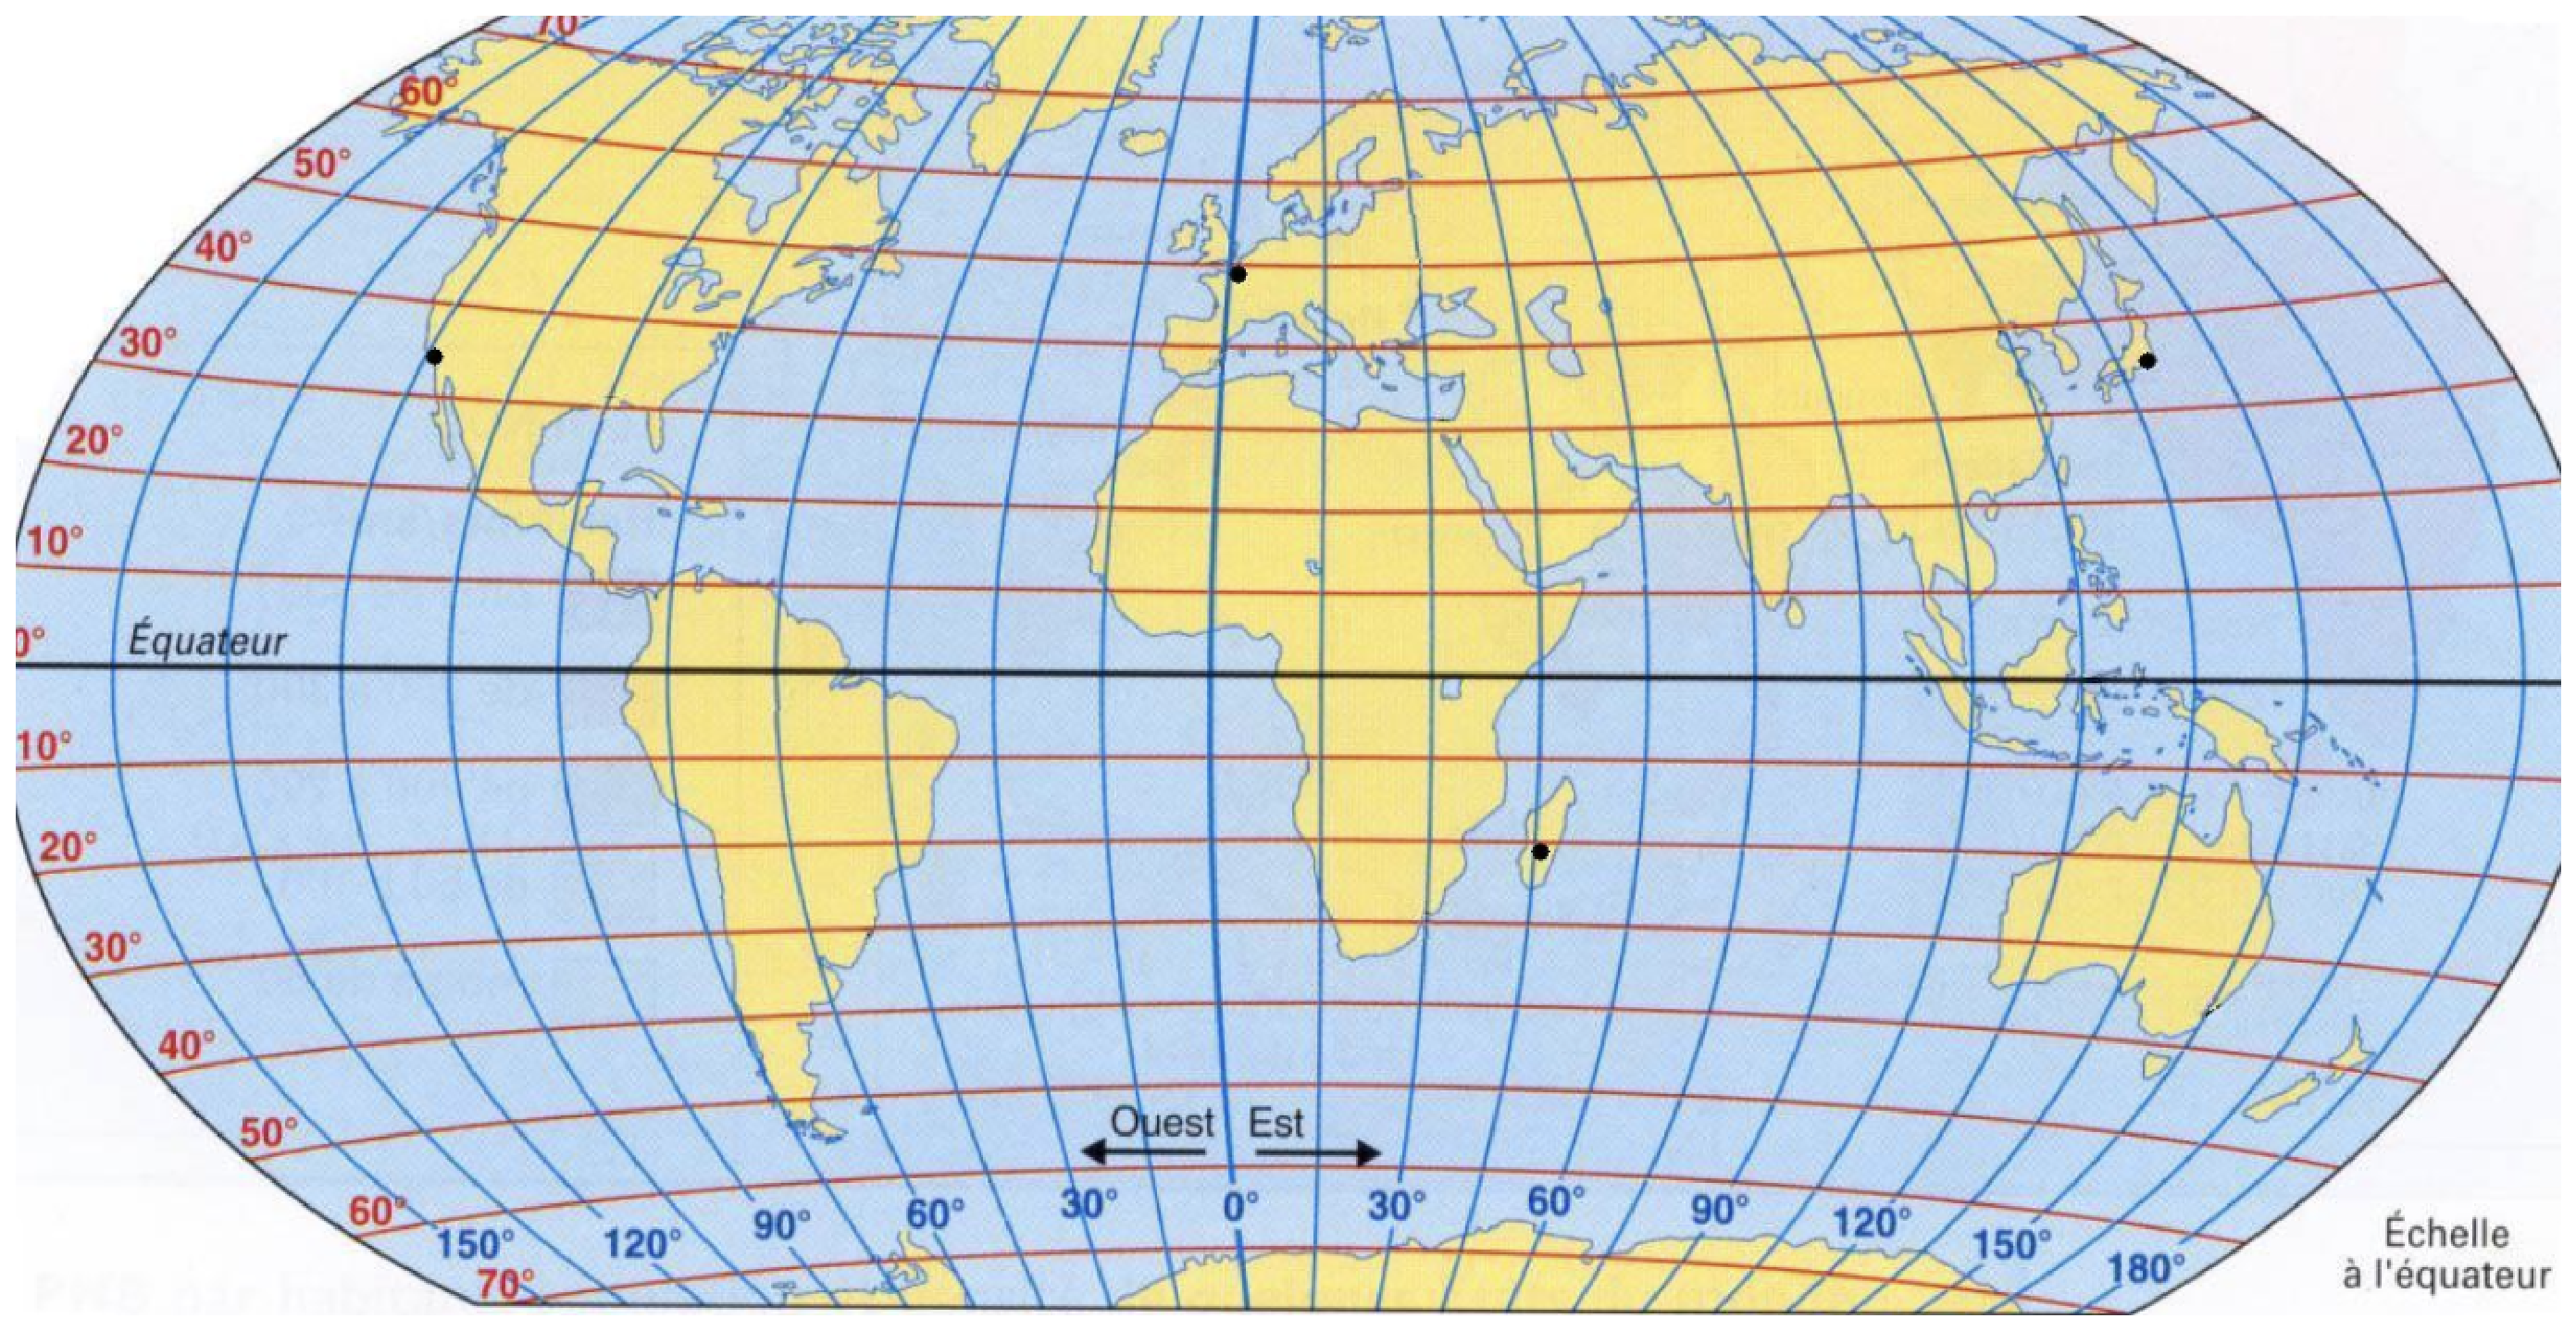
\includegraphics[width=14.cm]{Mappemonde_Metropole_sept_2021}}
\psdots[linecolor=yellow,dotscale=1.](2.8,6.7)(7.22,7.18)(8.9,4)(12.2,6.675)
\end{pspicture}
\end{center}
%%%%%  fin Métropole, Antilles--Guyane 13 septembre 2021
\newpage
%%%%%  Amérique du Sud 23 novembre 2021
\hypertarget{AmeriqueSud}

\label{AmeriqueSud}

\lfoot{\small{Amérique du Sud }}
\rfoot{\small{23 novembre 2021}}
\pagestyle{fancy}
\thispagestyle{empty}
\begin{center}

{\Large \textbf{\decofourleft~Brevet des collèges Amérique du Sud 23 novembre 2021~\decofourright}}

\bigskip

\textbf{Durée : 2 heures}

\end{center}

\medskip

\textbf{\large Exercice 1 \hfill 24 points}

\medskip

Pour chacune des six affirmations suivantes, indiquer si elle est vraie ou fausse.

On rappelle que toutes les réponses doivent être justifiées.\index{Vrai-Faux}

\begin{center}
\begin{tabularx}{\linewidth}{|X|}\hline
\textbf{Affirmation 1}: 72 est un multiple commun des nombres 12 et 18.\\ \hline\index{multiple}
\textbf{Affirmation 2} : pour tout nombre $n$, on a l'égalité suivante: $(n - 5)^2 = n^2 - 5^2$.\rule[-3mm]{0mm}{8mm}\\ \hline\index{identité}
On considère la fonction $f$ définie par $f(x) = 2x +5$.\\\index{fonction affine}
\textbf{Affirmation 3}: l'antécédent de 6 par la fonction $f$ est égal à $\dfrac{1}{2}$.\\ \hline
Voici les températures relevées en degré Celsius (noté \degres C) pendant six jours dans une même ville: 5~\degres C, 7~\degres C, 11~\degres C, 8~\degres C, 5~\degres C et 6~\degres C.\\\index{antécédent}
\textbf{Affirmation 4} : la moyenne de ces six températures est égale à 6,5~\degres C.\\ \hline
\parbox{0.48\linewidth}{Les points B, D et A sont alignés.\index{moyenne}

Les points B, E et C sont alignés.

Le triangle ABC est rectangle en B.

BA $= 12$ cm ; BC $= 9$ cm ;

BD $= 8$ cm et BE $= 6$ cm.

\emph{La figure ci-contre n'est pas à l'échelle.}}
\hfill \parbox{0.43\linewidth}{\psset{unit=0.6cm}
\begin{pspicture}(9.5,6.4)
\pspolygon(2.9,0)(9.5,0)(9.5,4)%DBE
\pspolygon(0,0)(9.5,0)(9.5,6)%ABC
\psframe(9.5,0)(9.2,0.3)
\uput[d](0,0){A}\uput[d](9.5,0){B}\uput[r](9.5,6){C}
\uput[d](2.9,0){D}\uput[r](9.5,4){E}
\end{pspicture}}\\
\textbf{Affirmation 5}: la longueur AC est égale à $15$~cm.\\
\textbf{Affirmation 6}: les droites (AC) et (DE) sont parallèles.\\ \hline\index{Thalès}
\end{tabularx}
\end{center}

\bigskip

\textbf{\large Exercice 2 \hfill 19 points}

\medskip

Une mère et sa fille rentrent chez elles à pied en empruntant le même trajet de
10 kilomètres. La mère décide de s'y rendre en marchant et sa fille en courant.

Le graphique ci-dessous modélise les parcours de la mère et de la fille depuis leur départ.

\begin{figure}
\begin{center}
\psset{xunit=4cm,yunit=1cm,arrowsize=2pt 3}
\begin{pspicture}(-0.25,-1)(2.25,10)
\multido{\n=0.00+0.25}{10}{\psline[linewidth=0.15pt](\n,0)(\n,10)}
\multido{\n=0+1}{11}{\psline[linewidth=0.15pt](0,\n)(2.25,\n)}
\psaxes[linewidth=1pt]{->}(0,0)(0,0)(2.25,10)
\psline[linecolor=blue,linewidth=1.5pt](0,0)(0.25,3)(0.75,3)(1.833,10)
\psline[linecolor=red,linestyle=dotted,linewidth=1.5pt](0,0)(2,10)
\uput[r](0,10.2){Distance parcourue (en km)}
\rput(0.5,4.5){\blue Parcours de la fille}\psline[linecolor=blue]{->}(0.5,4.2)(0.3,3)
\rput(0.75,1.2){\red Parcours de la mère}\psline[linecolor=red]{->}(0.6,1.3)(0.45,2.2)
\uput[u](1.85,0){Temps de parcours (en h)}
\end{pspicture}
\end{center}
\end{figure}

\medskip

\begin{enumerate}
\item 
	\begin{enumerate}
		\item Indiquer le temps mis par la mère pour rentrer chez elle, avec la précision que permet la lecture du graphique.\index{lecture graphique}
		\item Déterminer la vitesse moyenne en km/h de la mère sur l'ensemble de son parcours.\index{moyenne}
		\item La distance parcourue par la mère est-elle proportionnelle au temps ?
	\end{enumerate}
\item La fille est partie à $16$~h et est arrivée chez elle à $17$~h $50$. Elle a fait une pause durant sa course.
	\begin{enumerate}
		\item Indiquer la durée de la pause de la fille, avec la précision que permet la lecture graphique.
		\item Quand a-t-elle couru le plus vite: avant ou après sa pause ?
	\end{enumerate}
\item Combien de fois la mère et la fille se sont retrouvées au même endroit et au même moment, au cours de leur trajet ?
\item Dans cette question, on note $f$ la fonction qui, au temps de parcours $x$ (exprimé en heure) de la mère depuis le départ, associe la distance parcourue (exprimée en kilomètre) par la mère depuis le départ.

Parmi les propositions suivantes, recopier sans justification l'expression de $f(x)$ :

\[f(x) = \dfrac{1}{5}x \quad;\quad  f(x) = 5x \quad;\quad  f(x) = x + 5.\]\index{fonction linéaire}\index{fonction affine}

\end{enumerate}

\bigskip

\textbf{\large Exercice 3 \hfill 23 points}

\medskip

Un club de handball souhaite commander des maillots avec le nom du club inscrit dessus. À l'issue de sa commande, le club veut recevoir exactement $350$~maillots.

Après quelques recherches, deux sites internet ont été sélectionnés:

\setlength\parindent{1cm}
\begin{itemize}
\item[$\bullet~~$] sur le site A : les maillots sont vendus à 12~\euro{} l'unité;
\item[$\bullet~~$] sur le site B : les maillots sont vendus à 13~\euro{} l'unité, avec la promotion :

\begin{center}\og 10 maillots offerts pour 100 achetés \fg.\end{center}
\end{itemize}
\setlength\parindent{0cm}

\medskip

\begin{enumerate}
\item Déterminer le montant, exprimé en euro, de la commande du club envisagée sur le site A.
\item Un tableur ci-dessous présente des exemples de dépenses en fonction du nombre de maillots payés sur le site B. Voici une copie d'écran de ce tableur.\index{tableur}

\begin{center}
\begin{tabularx}{\linewidth}{|c|>{\small}p{4cm}|*{8}{>{\centering \arraybackslash}X|}}\hline
 &A								&B	&C	&D	&E		& F	& G	& H	&I\\ \hline 
1&Nombre de maillots payés		&50 &100&150&200 &250	&300&350&400\\ \hline
2&Nombre de maillots offerts	&0	&10	&10	&20	&20	&30	&30	&40\\ \hline
3&Nombre total de maillots reçus&50 &110 &160	&220	&270&330&380 &440\\ \hline
4&Coût total (en \euro)			&650&\np{1300}&\np{1950}&\np{2600}&\np{3250}&\np{3900}&\np{4550}& \np{5200}\\ \hline
\end{tabularx}
\end{center}

	\begin{enumerate}
		\item À la lecture de ce tableur, le trésorier du club affirme que le montant de la commande
sera compris entre \np{3900}~\euro{} et \np{4550}~\euro. Son affirmation est-elle vraie ?
		\item Sachant que les lignes 1 et 2 du tableur ont été complétées auparavant, quelle formule a-t-on pu saisir ensuite dans la cellule B3 avant de l'étirer jusqu'à la cellule I3, pour remplir la ligne 3 du tableur ?
		\item Le coût total exprimé en euro est-il proportionnel au nombre de maillots reçus ?
	\end{enumerate}
\item Sur quel site le club doit-il passer sa commande pour recevoir exactement $350$~maillots, tout en payant le moins cher ?
\item Le club souhaite que ces $350$~maillots soient répartis entre des maillots noirs et des maillots rouges dans le ratio 5 : 2.

Combien faut-il commander de maillots noirs et de maillots rouges ?
\item Le club a aussi commandé des gourdes. Les cartons reçus sont indiscernables tant par leurs dimensions que par leur forme. 

Il y a 4 cartons de gourdes blanches et 3 cartons de gourdes bleues.

On ouvre un carton au hasard. Quelle est la probabilité qu'il contienne des gourdes bleues ?\index{probabilité}
\end{enumerate}

\bigskip

\textbf{\large Exercice 4 \hfill 14 points}

\medskip

\emph{Dans tout cet exercice, aucune justification n'est demandée}

\smallskip

On donne le programme suivant :\index{scratch}

\begin{center}
\begin{tabular}{l l}
Script principal&le bloc Carré\\
\begin{scratch}
\blockinit{quand \greenflag est cliqué}
\blocklook{effacer tout}
\blockmove{aller à x: \ovalnum{0} y : \ovalnum{0}}
\blockmove{s'orienter à \ovaloperator{\selectmenu{90}}}
\blockrepeat{répéter \ovalnum{4} fois}
{\blockmoreblocks{Carré}
\blockmove{avancer de \ovalnum{50}}
}
\end{scratch}&\begin{scratch}
\initmoreblocks{définir \namemoreblocks{Carré}}
\blockpen{stylo en position d'écriture}
\blockrepeat{répéter \ovalnum{4} fois}
{\blockmove{avancer de \ovalnum{50}}
\blockmove{tourner \turnleft{} de \ovalnum{90} degrés}
}
\blockpen{relever le stylo}
\end{scratch}\\
\end{tabular}
\end{center}

On rappelle que l'instruction \begin{scratch}\blockmove{s'orienter à \ovalnum{90}}\end{scratch}
signifie que l'on s'oriente vers la droite.

\begin{enumerate}
\item On lance le programme.

Construire la figure obtenue en prenant 1 cm pour 25 unités de longueur.

\smallskip

On modifie le Script principal et on obtient deux scripts ci-dessous:

\begin{center}
\begin{tabular}{l l}
Script principal A&Script principal B\\
\begin{scratch}
\blockinit{quand \greenflag est cliqué}
\blocklook{effacer tout}
\blockmove{aller à x: \ovalnum{0} y : \ovalnum{0}}
\blockmove{s'orienter à \ovaloperator{\selectmenu{90}}}
\blockrepeat{répéter \ovalnum{3} fois}
{\blockmoreblocks{Carré}
\blockmove{avancer de \ovalnum{25}}
}
\end{scratch}&\begin{scratch}
\blockinit{quand \greenflag est cliqué}
\blocklook{effacer tout}
\blockmove{aller à x: \ovalnum{0} y : \ovalnum{0}}
\blockmove{s'orienter à \ovaloperator{\selectmenu{90}}}
\blockrepeat{répéter \ovalnum{4} fois}
{\blockmoreblocks{Carré}
\blockmove{tourner \turnleft{} de \ovalnum{90} degrés}
}
\end{scratch}\\
\end{tabular}
\end{center}

\item Parmi les trois figures ci-dessous, associer sur votre copie chacun des deux scripts principaux A et B à la figure qu'il permet de réaliser:

\begin{center}
\begin{tabularx}{\linewidth}{*{3}{>{\centering \arraybackslash}X}}
Figure 1 &Figure 2 &Figure 3\\
\psset{unit=1.25cm}
\begin{pspicture}(0,0)(2,2)
\psgrid[gridlabels=0pt,subgriddiv=1,gridwidth=1.2pt]
\end{pspicture}&\psset{xunit=0.6cm,yunit=1.2cm}
\begin{pspicture}(4,1)
\psgrid[gridlabels=0pt,subgriddiv=1,gridwidth=1.2pt]
\end{pspicture}&\psset{unit=1.25cm}
\begin{pspicture}(3,2)
\psgrid[gridlabels=0pt,subgriddiv=1,gridwidth=1.2pt]
\end{pspicture}\\
\end{tabularx}

\end{center}

\bigskip

On souhaite réaliser la figure suivante :

\begin{center}
\psset{unit=1cm}
\begin{pspicture}(-1.5,-1.5)(1.5,1.5)
\psframe(-1,-1)(1,1)\psline(-1,0)(1,0)\psline(0,-1)(0,1)
\rput{45}(0,0){\psframe(-1,-1)(1,1)\psline(-1,0)(1,0)\psline(0,-1)(0,1)}
\end{pspicture}
\end{center}

\smallskip

Le point de départ se situe au centre de la figure.
\item Compléter le nouveau script principal ci-dessous en recopiant sur la copie uniquement les lignes 5 et 7. Pour mémoire, l'énoncé rappelle ci-dessous à droite le descriptif du bloc Carré.

\begin{center}
\begin{tabular}{r l l}
Numéros de ligne \psset{arrowsize=2pt 3}\psline{->}(0,0)(0.55,-0.8)&Script principal&le bloc Carré\\
&\begin{scratch}[num blocks]
\blockinit{quand \greenflag est cliqué}
\blocklook{effacer tout}
\blockmove{aller à x: \ovalnum{0} y : \ovalnum{0}}
\blockmove{s'orienter à \ovaloperator{\selectmenu{90}}}
\blockrepeat{répéter \ovalnum{\ldots\ldots} fois}
{\blockmoreblocks{Carré}
\blockmove{\ldots\ldots\ldots}
}
\end{scratch}&\begin{scratch}
\initmoreblocks{définir \namemoreblocks{Carré}}
\blockpen{stylo en position d'écriture}
\blockrepeat{répéter \ovalnum{4} fois}
{\blockmove{avancer de \ovalnum{50}}
\blockmove{tourner \turnleft{} de \ovalnum{90} degrés}
}
\blockpen{relever le stylo}
\end{scratch}\\
\end{tabular}
\end{center}

\end{enumerate}

\bigskip

\textbf{Exercice 5 \hfill 20 points}

\medskip

Une usine de fabrication de bougies reçoit des cubes de cire d'abeille d'arête 6 cm.

Ils sont disposés dans des cartons remplis (sans espace vide).

\begin{center}
\begin{tabular}{l p{5mm} l}
\begin{tabular}{|p{5cm}|}\hline
\textbf{Informations sur les cartons:}\\
Forme: pavé droit\\ 
Dimensions : \\
\begin{itemize}
\item largeur : 60 cm
\item hauteur : 36 cm
\item profondeur : 36 cm
\end{itemize}\\
(On ne tient pas compte de l'épaisseur des cartons)\\ \hline
\end{tabular} &~&
\begin{tabular}{|p{5cm}|}\hline
\textbf{Information sur la cire d'abeille:}\\
Masse volumique: 0,95 g/cm$^3$\\ \hline
\end{tabular}
\end{tabular}
\end{center}

\medskip

\begin{enumerate}
\item 
	\begin{enumerate}
		\item Montrer que chaque carton contient 360 cubes de cire d'abeille.
		\item Quelle est la masse de cire d'abeille contenue dans un carton rempli de cubes? On donnera la réponse en kg, arrondie à l'unité près, en ne tenant pas compte de la masse du carton.
	\end{enumerate}
\item À l'usine, on découpe les cubes de cire d'abeille afin d'obtenir des cylindres de hauteur 6 cm et de diamètre 6 cm avec lesquels on fera des bougies en installant une mèche.

\begin{center}
\begin{tabular}{|*{5}{c}|}\hline
\psset{unit=1cm,arrowsize=15pt,arrowinset=0.8}
\begin{pspicture}(3,3)
%\psgrid
\pspolygon(0,0.6)(1,0)(2.7,0.3)(2.7,2.1)(1.7,2.8)(0,2.5)
\psline(2.7,2.1)(1,1.8)(0,2.5)\psline(1,0)(1,1.8)
\psline[linestyle=dotted](0,0.6)(1.7,0.9)(2.7,0.3)
\psline[linestyle=dotted](1.7,0.9)(1.7,2.8)
\end{pspicture}&\begin{pspicture}(1.5,3)\psline[linewidth=5pt,arrowsize=15pt,arrowlength=0.5,arrowinset=0.1]{->}(0,1.5)(1.5,1.5)\end{pspicture}&\begin{pspicture}(3,3)
\pspolygon(0,0.6)(1,0)(2.7,0.3)(2.7,2.1)(1.7,2.8)(0,2.5)
\psline(2.7,2.1)(1,1.8)(0,2.5)\psline(1,0)(1,1.8)
\psline[linestyle=dotted](0,0.6)(1.7,0.9)(2.7,0.3)
\psline[linestyle=dotted](1.7,0.9)(1.7,2.8)
\def\bougie{
\psset{unit=1cm}
\begin{pspicture}(-1,-0.5)(1,2.3)
\psline(-0.95,0)(-0.95,1.8)\psline(0.95,0)(0.95,1.8)
\psellipse(0,1.8)(0.95,0.4)
\psellipticarc[linewidth=1.25pt,linestyle=dotted](0,0)(0.95,0.4){0}{180}
\psellipticarc[linewidth=1.25pt](0,0)(0.95,0.4){180}{360}
\end{pspicture}}
\rput(1.28,1.43){\bougie}
\end{pspicture}&\begin{pspicture}(1.5,3)\psline[linewidth=5pt,arrowsize=15pt,arrowlength=0.5,arrowinset=0.1]{->}(0,1.5)(1.5,1.5)\end{pspicture}&
\begin{pspicture}(-1,-0.5)(1,2.3)
%\psgrid
\psline(-1,0)(-1,2)\psline(1,0)(1,2)
\psellipse(0,2)(1,0.37)
\psellipticarc[linewidth=1.25pt,linestyle=dotted](0,0)(1,0.37){0}{180}
\psellipticarc[linewidth=1.25pt](0,0)(1,0.37){180}{360}
\end{pspicture}\\
Cube de cire	&&&&Bougie cylindrique\\
d'abeille		&&&&(sans sa mèche)\\
Arête: 6 cm		&&&& Hauteur : 6 cm\\
				&&&& Diamètre: 6 cm\\ \hline
\end{tabular}
\end{center}

\emph{On ne tiendra pas compte de la masse, du volume et du prix de Ja mèche dans la suite de l'exercice.}

\medskip

	\begin{enumerate}
		\item Montrer que le volume d'une bougie est d'environ $170$~cm$^3$.\index{volume}
		
		\smallskip
		
On rappelle que le volume d'un cylindre de rayon $r$ et de hauteur $h$ est donné par la formule :

\[V = \pi \times  r^2 \times h.\]

		\item En découpant les cubes de cire d'abeille d'arête 6~cm pour former des bougies cylindriques, la cire perdue est réutilisée pour former à nouveau d'autres cubes de cire d'abeille d'arête 6~cm. 
		
Combien de cubes au départ doit-on découper pour pouvoir reconstituer un cube de cire d'abeille d'arête 6~cm, avec la cire perdue ?
	\end{enumerate}
\item Un commerçant vend les bougies de cette usine au prix de $9,60$~\euro{} l'unité. Il les vend 20\,\% plus chères qu'il ne les achète à l'usine.\index{pourcentage}

Combien paie-t-il à l'usine pour l'achat d'une bougie ?
\end{enumerate}
%%%%%  fin Amérique du Sud 23 novembre 2021
\newpage
%%%%%  Nouvelle-Calédonie 7 décembre 2021
\hypertarget{Caledoniedec}{}

\label{Caledoniedec}

\lfoot{\small{Nouvelle-Calédonie}}
\rfoot{\small{7 décembre 2021}}
\marginpar{\rotatebox{90}{\textbf{A. P{}. M. E. P{}.}}}
\pagestyle{fancy}
\thispagestyle{empty}

\begin{center}\textbf{Durée : 2 heures}

\vspace{0,5cm}

{\Large\textbf{\decofourleft~Diplôme national du Brevet
Nouvelle--Calédonie~\decofourright}}\\[7pt]
{\Large \textbf{7 décembre 2021}}
\end{center}

\vspace{0,5cm}

\textbf{Exercice 1 : \hfill 18 points}

\medskip

Pour chaque affirmation répondre par vrai ou faux. Justifier chaque réponse.\index{Vrai-Faux}

\medskip

\textbf{Affirmation 1 :} 50\,\% de \np{10350} c'est \np{10300}.\index{pourcentage}

\medskip

\textbf{Affirmation 2 :} $\dfrac73$ est la forme irréductible de $\dfrac{42}{18}$.

\medskip

\textbf{Affirmation 3 :} L'équation $2x - 4 = -x + 5$ a pour solution $3$.\index{equation@équation}

\medskip

\textbf{Affirmation 4 :} L'arrondi à l'unité près du volume d'une boule de diamètre $21,6$~cm est \np{42213}~cm$^3$.\index{volume}

\smallskip

\emph{On rappelle la formule du volume d'une boule } $V = \dfrac43 \pi R^3$.

\medskip

\begin{minipage}{0.52\linewidth}
\textbf{Affirmation 5 :} Dans la figure codée ci-contre, la  mesure de l'angle $\widehat{\text{DNB}}$, arrondie à l'unité près, est $18\degres$.
\end{minipage}\hfill
\begin{minipage}{0.38\linewidth}
\psset{unit=1cm}
\begin{pspicture}(5.5,2.4)
\pspolygon(0.4,0.2)(5.1,0.2)(0.4,1.9)%BND
\psframe(0.4,0.2)(0.6,0.4)
\uput[dl](0.4,0.2){B} \uput[dr](5.1,0.2){N} \uput[u](0.4,1.9){D} \uput[l](0.4,1.05){4 cm} \uput[d](2.75,0.2){12 cm}
\end{pspicture}
\end{minipage}

\bigskip

\textbf{Affirmation 6 :} On peut composer 6 codes différents avec un cadenas à 3 chiffres qui respecte les conditions suivantes :

\begin{itemize}
\item[$\bullet~~$]les deux premiers chiffres sont choisis parmi 1 ; 2 et 3 ;
\item[$\bullet~~$]un chiffre peut apparaître deux fois;
\item[$\bullet~~$]le dernier chiffre est 6.
\end{itemize}

\bigskip

\textbf{Exercice 2 : \hfill 10 points}

\medskip

On étudie les précipitations (hauteurs de pluies) sur la ville de Nouméa entre avril et décembre 2020. 

On obtient le tableau suivant:

\begin{center}
\begin{tabularx}{\linewidth}{|m{3.5cm}|*{9}{>{\centering \arraybackslash}X|}}\hline
Mois 				&Avril 	&Mai &Juin 	&Juillet &Août 	&Sept 	&Oct &Nov 	&Déc.\\ \hline
Précipitations en mm&147 	&199 &40 	&67 	&47 	&54 	&104 &45 	&63\\ \hline
\multicolumn{10}{r}{\footnotesize Source: https://www.historigue-meteo.net/oceanie/nouvelle-caledonie/noumea/2020}\\
\end{tabularx}
\end{center}

\medskip

\begin{enumerate}
\item Calculer la moyenne des précipitations. Arrondir le résultat au mm près.\index{moyenne}
\item Quelle est l'étendue des précipitations ?\index{etendue@étendue}
\item Déterminer la médiane des précipitations.\index{médiane}
\item Calculer le pourcentage de mois pour lesquels les précipitations sont supérieures à $100$~mm. Arrondir le résultat à l'unité près.\index{pourcentage}
\end{enumerate}

\bigskip

\textbf{Exercice 3 : \hfill 10 points}

\medskip

BAI est un triangle rectangle en A tel que BA $= 210$~cm et AI $= 155$~cm. 

\medskip

\begin{enumerate}
\item Déterminer la longueur BI au cm près.\index{Pythagore}

\textbf{Rédiger la réponse en faisant apparaître les différentes étapes.}

L'immeuble de Joanne possède 15 vitres rectangulaires.

Chaque vitre a pour longueur 210 cm et pour largeur 155 cm.

Lors d'une préalerte cyclonique Joanne pose de l'adhésif sur les deux diagonales de chaque vitre de l'immeuble.
\begin{center}
\psset{unit=1cm,arrowsize=2pt 3}
\begin{pspicture}(6,6.8)
%\psgrid
\psframe(1.5,1.8)(4.5,6.3)
\psline(1.5,1.8)(4.5,6.3)\psline(4.5,1.8)(1.5,6.3)
\uput[d](3,6.3){$155$~cm}\uput[r](4.5,4.05){210 cm}
\rput(3,0.2){Une bande d'adhésif est assimilée à une diagonale du rectangle}
\rput(3,6.6){Schéma de la situation}
\psline{->}(3,0.6)(2.3,3)\psline{->}(3,0.6)(3.7,3)
\end{pspicture}
\end{center}

\item Justifier que Joanne a besoin d'environ $5,22$ m d'adhésif pour une vitre.
\end{enumerate}

Joanne a 7 rouleaux d'adhésif de $10$ m chacun.

\begin{enumerate}[resume]
\item A-t-elle assez d'adhésif pour toutes les vitres ? Justifier la réponse.
\end{enumerate}

\bigskip

\textbf{Exercice 4 : \hfill 14 points}

\medskip

\begin{enumerate}
\item 
	\begin{enumerate}
		\item Justifier que $330$ n'est pas un nombre premier.
		
La décomposition en produit de facteurs premiers de $500$ est: $500 = 2^2 \times 5^3$.
		\item Décomposer $330$ en produit de facteurs premiers.\index{produit de facteurs premiers}
		\item Justifier que $165$ divise $330$.
		\item Justifier que 165 ne divise pas $500$.
	\end{enumerate}
\end{enumerate}
	
La pâtisserie Délices a préparé $330$ biscuits aux noix et $500$ biscuits au chocolat.

\textbf{La pâtisserie souhaite répartir le plus de biscuits possible dans $165$ boites.}

La pâtisserie met le même nombre de biscuits aux noix dans chaque boîte.\index{pgcd}

\begin{enumerate}[resume]
\item Combien de biscuits aux noix y a-t-il dans chaque boîte ?

La pâtisserie met aussi le même nombre de biscuits au chocolat dans chaque boîte.
\item
	\begin{enumerate}
		\item Combien de biscuits au chocolat y a-t-il dans chaque boîte ?
		\item Combien de biscuits au chocolat reste-t-il ?
	\end{enumerate}
		
Une boîte de biscuits coûte \np{3650} francs.

À partir de 10 boîtes achetées, la pâtisserie Délices offre une réduction de 5\,\% sur le montant total.
\item Combien va-t-on payer pour l'achat de 12 boîtes ?\index{pourcentage}

Faire apparaÎtre les calculs effectués.

\end{enumerate}

\bigskip

\textbf{Exercice 5 : \hfill 18 points}

\medskip

Un jeu est constitué de quatre familles de cartes:
banane ; 
prune ; 
citron ;
fraise.

Voici la répartition des cartes de la famille banane.

\begin{center}
\begin{tabularx}{\linewidth}{|m{3.5cm}|*{5}{>{\centering \arraybackslash}X|}}\hline
Nombre de banane(s)	&1&2&3&4&5\\ \hline
Nombre de cartes	&5&3&3&2&1\\ \hline
\end{tabularx}
\end{center}

La répartition est la même pour les cartes avec les autres fruits.

\medskip

\begin{enumerate}
\item Montrer que ce jeu a $56$ cartes.

Joanne mélange toutes les cartes. Son frère Jack prend une carte au hasard. On admet que chaque carte a la même chance d'être choisie.

Soit $P$ l'évènement: \og Jack obtient une carte de la famille prune \fg.
\item Quelle est la probabilité de l'évènement $P$ ?\index{probabilité}
\item 
	\begin{enumerate}
		\item Quel est l'évènement contraire de $P$ ?
		\item Quelle est la probabilité de l'évènement contraire de $P$ ?
	\end{enumerate}	
\item Quelle est la probabilité d'obtenir une carte avec quatre fruits ?
\end{enumerate}

\bigskip

\textbf{Exercice 6 : \hfill 14 points}

\medskip

\textbf{Les parties 1 et 2 sont indépendantes}

\bigskip

\textbf{Partie 1 : Distance de réaction}

\medskip

La distance de réaction d'un véhicule est la distance parcourue par ce véhicule entre l'instant où le conducteur voit un obstacle et l'instant où il appuie sur la pédale de frein.

On considère un conducteur en bonne santé.

La distance de réaction, en mètre, en fonction de la vitesse du véhicule est représentée par le graphique de l'annexe.

\medskip

\begin{enumerate}
\item Cette représentation graphique traduit-elle une situation de proportionnalité ?\index{fonction linéaire}

Justifier la réponse.
\item Compléter, par lecture graphique, le tableau de l'annexe.\index{lecture graphique}
\end{enumerate}

\bigskip

\textbf{Partie 2 : Distance de freinage sur route sèche}

\medskip

La distance de freinage d'un véhicule est la distance parcourue par ce véhicule entre l'instant où le conducteur appuie sur la pédale de frein et l'instant où la voiture s'arrête complètement.

La distance de freinage en mètre, pour un véhicule en bon état, est déterminée en fonction de la vitesse du véhicule par la formule :

\begin{center}$d = \dfrac{v^2}{203,2}$ \:  où $v$ est la vitesse exprimée en km/h\end{center}

On utilise un tableur  pour calculer les distances de freinage en fonction de la vitesse :\index{tableur}

\begin{center}
\begin{tabularx}{\linewidth}{|c|m{3.5cm}|*{3}{>{\centering \arraybackslash}X|}}\hline
&A&B&C&D\\ \hline
1 &vitesse (km/h) &10 &20 &30\\ \hline
2 &distance de freinage (m)&&&\\ \hline
\end{tabularx}
\end{center}

\medskip

\begin{enumerate}
\item Recopier parmi les formules trois suivantes, celle qu'il faut saisir dans la cellule B2 puis étirer vers la droite:

\begin{center}\fbox{= 2*B1/203.2}\qquad  \fbox{= B1*B1/203.2} \qquad  \fbox{= B1+B1/203.2}\end{center}

\item Un véhicule roule à $90$ km/h. 

Montrer que sa distance de freinage est environ $40$~m.

\end{enumerate}

\bigskip

\textbf{Partie 3 : Distance d'arrêt sur route sèche}

\medskip

La distance d'arrêt d'un véhicule est la distance parcourue par ce véhicule entre l'instant où le conducteur voit un obstacle et l'instant où la voiture s'arrête complètement.

Distance d'arrêt = Distance de réaction $+$ Distance de freinage

Calculer la distance d'arrêt d'un véhicule roulant à $90$ km/h.

\bigskip

\textbf{Exercice 7 : \hfill 9 points}

\medskip

On doit appliquer deux couches de peinture sur le sol et les parois intérieures d'une piscine rectangulaire dont les dimensions sont données dans le document 2.

À l'aide des documents ci-dessous, calculer le budget que l'on doit prévoir pour les travaux de peinture.\index{aire}

\begin{center}
\begin{tabularx}{\linewidth}{|m{5.6cm}|X|}\hline
\textbf{Document 1 :} pot de peinture

Surface pouvant être peinte: $35$ m$^2$

Prix : \np{12000}~F&
\textbf{Document 2 :} piscine de base rectangulaire 

Longueur : 8~m Largeur : 4~m Profondeur : 1,70~m

\begin{center}
\psset{unit=0.8cm}
\begin{pspicture}(0,-1.4)(7.8,3.5)
%\psgrid
\pspolygon(0,1.4)(5.8,0)(6.5,2.3)(0.7,3.7)
\psline(0.7,3.7)(0.7,2.3)(6.1,1)
\psline(0,1.4)(0,0)(5.8,-1.4)(5.8,0)
\psline(5.8,-1.4)(6.5,0.9)(6.5,2.3)
\psline(0.7,2.3)(0.4,1.3)
\rput(3.6,3.4){8 m}
\rput(0,2.8){4 m}
\uput[r](6.5,1.6){1,70 m}
\end{pspicture}
\end{center}\\ \hline
\end{tabularx}
\end{center}

\textbf{Toute trace de recherche même non aboutie sera prise en compte dans la notation.}

\bigskip

\textbf{Exercice 8: \hfill 13 points}

\medskip

%La photo ci-dessous montre le phare Amédée, une balise et une bouée :

%\begin{center}\includegraphics[width=12cm]{phare_7_12_2021} \end{center}

On dispose des informations suivantes sur le phare Amédée, une balise et une bouée :

\begin{itemize}
\item la hauteur du phare est de $56$~m ;
\item la balise est située à $260$~m du phare;
\item la balise et la bouée sont distantes de $151$~m ;
\item la bouée O, le sommet B de la balise et le sommet P du phare sont considérés comme trois points alignés.
\end{itemize}

Schéma de la situation :

\begin{center}
\psset{unit=1cm,arrowsize=2pt 3}
\begin{pspicture}(10.5,3.5)
\psline(0,0.5)(10,0.5)(0,3.1)%HOP
\psline[linestyle=dashed](1.3,0.5)(1.3,2.7)
\psline[linestyle=dashed](7.1,0.5)(7.1,1.25)
\uput[u](1.3,2.7){P} \uput[d](1.3,0.5){H} \uput[u](7.1,1.25){B} \uput[d](7.1,0.5){A}
\uput[d](10,0.5){O} \uput[l](1.3,1.6){56 m} \uput[d](4.2,0.5){260 m} \uput[d](8.55,0.5){151 m}
\rput{90}(1.6,1.6){Phare} \rput{90}(7.4,0.85){Balise}\rput{90}(10,1){Bouée}
\psline[linewidth=0.6pt]{<->}(1.3,0)(7.1,0)
\psline[linewidth=0.6pt]{<->}(10,0)(7.1,0)
\end{pspicture}
\end{center}

\textbf{Les droites (PH) et (BA) sont parallèles.}

\medskip

\begin{enumerate}
\item Quelle est la distance OH en m ?
\item Déterminer la hauteur AB de la balise. Arrondir au dixième de m près.\index{Thalès}

\textbf{Rédiger la réponse en faisant apparaître les différentes étapes.}
\end{enumerate}

Le haut du phare est protégé par une barrière composée de sculptures.

\begin{center}
Contour de la sculpture
\medskip

\psset{unit=1cm,arrowsize=2pt 3}
\begin{pspicture}(-1.5,-1.5)(1.5,1.5)
\pspolygon(0.9;0)(1.4;15)(0.9;30)(1.1;45)(0.9;60)(1.4;75)(0.9;90)(1.1;105)(0.9;120)(1.4;135)(0.9;150)(1.1;165)(0.9;180)(1.4;195)(0.9;210)(1.1;225)(0.9;240)(1.4;255)(0.9;270)(1.1;285)(0.9;300)(1.4;315)(0.9;330)(1.1;345)
\end{pspicture}
\end{center}

On souhaite réaliser un programme Scratch pour reproduire le contour de cette sculpture.\index{scratch}
\begin{enumerate}[resume]
\item Calculer la mesure de l'angle $\widehat{a}$ en degré dans la figure ci-dessous:

\begin{center}
\psset{unit=1cm,arrowsize=2pt 3}
\begin{pspicture}(-1.5,-1.5)(1.5,1.5)
\psline[linestyle=dotted,linewidth=1.5pt](-1.5,0)(1.5,0)
\psline[linestyle=dotted,linewidth=1.5pt](0,0)(1.5;-72)
\psarc(0,0){0.5}{298}{360}\psarc(0,0){0.6}{0}{180}\psarc(0,0){0.5}{180}{288}\psarc(0,0){0.45}{180}{288}
\rput(0.9;90){$180\degres$}\rput(0.8;334){$72\degres$}\rput(0.75;234){$\widehat{a}$}
\psline(-0.6,0)(0,0)(0.5;288)
\end{pspicture}
\end{center}

Le script 1 permet de tracer le motif en pointillé ci-dessous (on part du point A et on s'arrête au point B).

\begin{center}
\psset{unit=1cm,arrowsize=2pt 3}
\begin{pspicture}(4.6,6)
%\psgrid
\psline(2.5,0)(0.2,0.3)(2.2,1.9)(1.1,3.2)(2.7,3.4)(2.4,5.5)(4.4,4.2)
\uput[l](0.2,0.3){B}\uput[r](0.4,0.45){$36\degres$}
\uput[r](1.2,3.1){$72\degres$}\uput[u](1.8,3.3){28}\uput[dl](1.6,2.6){28}
\uput[l](2.5,4.5){38}\uput[ul](2.2,5.5){A}\uput[ur](3.4,4.8){38}\uput[ul](1.2,1.18){38}
\uput[dl](1.4,0.1){38}
\rput{126}(2.2,1.9){\psframe(0.2,0.2)}
\rput{98}(2.7,3.4){\psframe(0.2,0.2)}
\end{pspicture}
\end{center}

\item Compléter le script 1 de l'annexe.
\end{enumerate}

Le script final permet de réaliser le contour de la sculpture.

\begin{enumerate}[resume]
\item Compléter le script final de l'annexe.
\end{enumerate}

\newpage

\begin{center}
\textbf{ANNEXE À RENDRE AVEC LA COPIE}
\end{center}
\medskip

\textbf{Exercice 6}

\medskip

\begin{center}
\psset{xunit=0.1cm,yunit=0.2cm,arrowsize=2pt 3}
\begin{pspicture}(-10,-2.5)(120,40)
\multido{\n=0+2}{61}{\psline[linewidth=0.1pt](\n,0)(\n,35)}
\multido{\n=0+1}{36}{\psline[linewidth=0.1pt](0,\n)(120,\n)}
\uput[r](0,36.5){Distance (m)}\uput[u](105,0){Vitesse (km/h)}
\rput(60,38){Distance de réaction en fonction de la vitesse}
\psaxes[linewidth=1.25pt,Dx=10,Dy=5]{->}(0,0)(0,0)(120,35)
\psplot[plotpoints=500,linewidth=1.25pt,linecolor=blue]{0}{110}{0.27777 x mul}
\end{pspicture}
\end{center}
\bigskip

\begin{center}
\begin{tabularx}{\linewidth}{|l| *{3}{>{\centering \arraybackslash}X|}}\hline
Vitesse (km/h)			&0 		&\ldots	&90\\ \hline
Distance de réaction (m)&\ldots	&15		&\ldots\\ \hline
\end{tabularx}
\end{center}

\bigskip

\textbf{Exercice 8 :}

\begin{center}
\begin{tabularx}{\linewidth}{XX}
\textbf{Script 1} &\textbf{Script final}\\
\begin{scratch}
\initmoreblocks{définir \namemoreblocks{motif}}%
\blockmove{avancer de \ovalnum{38} pas}
\blockmove{tourner \turnright{} de \ovalnum{} degrés}
\blockmove{avancer de \ovalnum{28} pas}
\blockmove{tourner \turnleft{} de \ovalnum{108} degrés}
\blockmove{avancer de \ovalnum{} pas}
\blockmove{tourner \turnright{} de \ovalnum{90} degrés}
\blockmove{avancer de \ovalnum{} pas}
\end{scratch}&
\begin{scratch}
\blockinit{Quand \greenflag est cliqué}
\blockpen{effacer tout}
\blockpen{stylo en position d'écriture}
\blockrepeat{répéter \ovalnum{} fois}
{
\blocklook{motif}
\blockmove{tourner \turnleft{} de \ovalnum{90} degrés}
}
\end{scratch}
\end{tabularx}
\end{center}
%%%%%  fin Nouvelle-Calédonie 7 décembre 2021
\phantomsection
\hypertarget{Index}{}
\setlength{\columnsep}{1.5cm}
\printindex
\end{document}